\documentclass{article}
\usepackage{iclr2027_conference,times}
\usepackage{microtype}
\usepackage{graphicx}
\usepackage{booktabs}
\usepackage{xurl}
\usepackage{hyperref}
\usepackage{amsmath,amssymb,amsthm,mathtools}
\usepackage{xcolor}
\usepackage{float}
\usepackage{enumitem}
\usepackage{array}
\usepackage{longtable}
\usepackage{adjustbox}
\newcommand{\zied}[1]{\textcolor{blue}{#1}}
\newcommand{\nat}[1]{\textcolor{red}{#1}}
\newcommand{\R}{\mathbb{R}}
\newcommand{\TOU}{\textsc{Ref}}
\newcommand{\RUNNING}{\zied{not verified}}
\DeclareMathOperator{\range}{range}
\DeclareMathOperator{\rank}{rank}
\DeclareMathOperator{\tr}{tr}
\DeclareMathOperator{\diag}{diag}
\newtheorem{proposition}{Proposition}
\newtheorem{lemma}[proposition]{Lemma}
\newtheorem{theorem}[proposition]{Theorem}
\theoremstyle{definition}
\newtheorem{definition}[proposition]{Definition}
\theoremstyle{remark}
\newtheorem{remark}[proposition]{Remark}
\graphicspath{{images/}}
\title{Diagnosing How Optimisers Shape Learning}
\author{Anonymous authors}
\hypersetup{hidelinks,pdftitle={Diagnosing How Optimisers Shape Learning},pdfauthor={Anonymous Authors},pdfsubject={ICLR 2027 submission draft},pdfkeywords={optimisation, implicit bias, neural networks, Jacobians}}
% Keep review mode; do not enable \iclrfinalcopy for submission.
\begin{document}
\maketitle

\begin{abstract}
Loss and accuracy track learning, but do not identify how a parameter update changes the function being learned. We introduce an operator-projection framework for diagnosing this process in bias-free piecewise-linear networks. At each training state, we separate the functional change that the current network can realise, the direction that the optimiser takes within this space, and parameter motion invisible to the sampled operators to first order. The reference is a diagnostic instrument, not a proposed optimisation algorithm. Studies of deep linear networks and MNIST-1D classifiers connect these local measurements to the evolution of gates and operator structure. Low alignment coexists with nearly complete estimated reachability. A reference-following control reduces input-dependent gating even with nonzero activation slopes; its ReLU operator participation ratio falls from \nat{$6.37$ to $3.28$ after training loss reaches $6.7\cdot10^{-7}$}. \nat{[Needs rewording: after class-centring, which removes the prediction-irrelevant common-logit direction, this decline is only $6.5\to5.4$ and the across-input diversity does not decline at all; see Section~\ref{sec:experiments}.]} Interventions on reference following and optimiser order further separate instantaneous update geometry from predictive performance. Together, these analyses connect optimiser updates to changes in the learned function, complementing loss, accuracy and structural learning curves.
\end{abstract}

\section{Introduction}
\label{sec:intro}

Two parameter updates can produce the same first-order decrease in training loss while changing different parts of a network's function. Conversely, they can produce the same local functional change while moving the parameters in different directions. These distinctions matter when interpreting learning. A loss curve records progress on the objective; test accuracy measures predictive performance; a rank statistic describes the structure of the current model. Understanding an optimiser additionally requires an account of how its parameter updates become changes in the function, and how those changes develop during training.

For deep linear networks, this conversion can be analysed through the end-to-end matrix. Gradient descent on the factors induces a depth-dependent transformation of the end-to-end gradient \citep{saxe2014exact,arora2018optimization,arora2019implicit}. Bias-free piecewise-linear networks retain a related description: for each input, the network computes $f_W(x)=P_W(x)x$, where $P_W(x)$ is its input Jacobian almost everywhere. The collection of these local operators describes both how the network responds to input perturbations and how its linear action varies across inputs. Following their changes offers a common setting in which to examine SGD, adaptive methods and matrix-preconditioned updates.

The difficulty is that the operators cannot move independently. They share the same weights, and their attainable changes depend on the current gates and factors. An update may therefore fail to follow an operator-gradient target because part of that target is locally inaccessible, because the optimiser favours a different attainable direction, or both. Low alignment alone cannot identify which explanation applies. The parameter update adds another ambiguity: some of its motion may leave all sampled operators unchanged to first order. Treating these effects as one undifferentiated ``bias'' obscures how an optimiser acts.

We address this problem with an \emph{operator-projection diagnosis}. We linearise the map from parameters to sampled operators, project an operator-gradient target onto its range, and use the minimum-norm lift of that projection as a reference. This separates local reachability, steering within the reachable space, and locally invisible parameter motion. A worked example shows how different operator directions and parameter routes can produce the same first-order loss decrease. The reference gives a precise meaning to the comparison; following it more closely is not the objective of the study. Our objective is to understand how an optimiser transforms the learning signal and how that transformation relates to the structures that emerge during training.

The experiments develop this account from local updates to learning trajectories. SGD can have low operator alignment even when the target is estimated to be fully reachable, revealing the steering induced by the parameterisation. Across activation functions, a trained reference-following control reduces input-dependent gating, including when every activation slope is nonzero. Along its trajectory, substantial operator complexity persists during fitting and then falls: an endpoint alone would hide this temporal distinction. Finally, changing the strength of reference following and the order of optimisation rules separates local alignment from prediction quality and exposes dependence on the state established earlier in training. These findings give the diagnostics an explanatory purpose: they identify differences in \emph{how learning proceeds}, which need not coincide with a ranking of optimisers by accuracy.

\section{From parameter updates to functional changes}
\label{sec:method}

\subsection{The operator target}

We consider a bias-free chain $W=(W_1,\ldots,W_L)$ with piecewise-linear, positively homogeneous activations and a linear output. At an input $x\in\R^d$, its operator is
\begin{equation}
 P_W(x)=W_LD_{L-1}(x)W_{L-1}\cdots D_1(x)W_1\in\R^{C\times d},
 \label{eq:operator}
\end{equation}
where $D_\ell(x)$ is the activation gate. Thus $f_W(x)=P_W(x)x$, and $P_W(x)$ equals the input Jacobian away from activation boundaries. Linear networks have $D_\ell=I$; ReLU and leaky ReLU have diagonal gates, with slopes in $\{0,1\}$ and $\{0.1,1\}$ in our experiments. CReLU concatenates positive and negative rectified responses \citep{shang2016crelu}, so its gate is rectangular and doubles the feature dimension. We keep pre- and post-activation dimensions distinct; Appendix~\ref{app:theory} gives the shapes and the convention at zero pre-activations.

For a batch $\{(x_i,y_i)\}_{i=1}^B$, write $\mathcal L=B^{-1}\sum_i\ell(f_W(x_i),y_i)$. We equip sampled operator collections with the average Frobenius inner product,
\begin{equation}
 \langle H,K\rangle_{\mathcal H}=\frac1B\sum_i\tr(H_i^\top K_i),
 \label{eq:metric}
\end{equation}
and parameter increments with the sum of layerwise Frobenius inner products, denoted $\langle\cdot,\cdot\rangle_{\mathcal W}$. If $g_i=\nabla_{f_i}\ell(f_i,y_i)$, the loss gradient with respect to independently varying sampled operators is $G_i=g_i x_i^\top$. We take the corresponding gradient step as the target:
\begin{equation}
 b=(b_i)_{i=1}^B,\qquad b_i=-\eta G_i,\qquad \eta>0.
 \label{eq:target}
\end{equation}
For half-squared loss, $g_i=f_i-y_i$; for cross-entropy, $g_i=\operatorname{softmax}(f_i)-e_{y_i}$. This target specifies what the loss requests in a declared operator metric. Input rescaling or a different metric can change the request; the reference is interpreted relative to this choice.

\subsection{What the current network can realise}

Let $A_{\ell,i}$ and $B_{\ell,i}$ be the products after and before $W_\ell$, including the appropriate gates, so that $P_W(x_i)=A_{\ell,i}W_\ell B_{\ell,i}$. At fixed gates, the local parameter-to-operator map and its adjoint are
\begin{align}
 (Mu)_i&=\sum_{\ell=1}^L A_{\ell,i}u_\ell B_{\ell,i},\label{eq:stepmap}\\
 (M^*H)_\ell&=\frac1B\sum_i A_{\ell,i}^\top H_iB_{\ell,i}^\top.
 \label{eq:adjoint}
\end{align}
In particular, $\nabla_W\mathcal L=M^*G$. When all sampled pre-activations are nonzero, a sufficiently small neighbourhood preserves their signs and
$P_{W+u}-P_W=Mu+O(\|u\|_{\mathcal W}^2)$. A gate crossing can make the operator jump, even though the output remains continuous. The diagnosis therefore concerns the local derivative; finite-step agreement is a separate empirical check.

The range of $M$ contains the jointly attainable operator changes. For example, inputs sharing a complete gate pattern have identical operators and local step maps, so the network cannot independently fulfil different operator requests on those inputs. Width or a large parameter count alone does not remove this coupling. Let $\Pi$ be orthogonal projection onto $\range(M)$. We define
\begin{equation}
 r=\Pi b,\qquad u^{\rm ref}=M^+b
 =\underset{u:\,Mu=r}{\arg\min}\|u\|_{\mathcal W}.
 \label{eq:reference}
\end{equation}
The projected target $r$ is the closest locally attainable request; $u^{\rm ref}$ selects its minimum-norm parameter representative. These two objects let us compare functional motion and the parameter route separately.

For a deep linear chain, every input shares the same operator. With $\bar b=B^{-1}\sum_i b_i$ and the single-operator map $M_0$, the reference has the exact linearised expression
\begin{equation}
 u^{\rm ref}=M_0^*T^+\bar b,\qquad
 T(H)=M_0M_0^*H=\sum_\ell A_\ell A_\ell^\top H B_\ell^\top B_\ell.
 \label{eq:transfer}
\end{equation}
Appendix~\ref{app:linear} derives this reduction and its rank conditions. It solves the local least-squares problem, not a finite factorisation constraint. In particular, the first-order reference is zero at all-zero weights of a linear chain of depth greater than one.

\section{Reading an optimiser through the diagnosis}
\label{sec:diagnostics}

\subsection{Reachability, steering and parameter motion}

For an optimiser's candidate increment $u$, define
\begin{align}
 \alpha&=\frac{\|r\|_{\mathcal H}}{\|b\|_{\mathcal H}}, &
 c_{\rm op}&=\cos_{\mathcal H}(Mu,r),\nonumber\\
 c_{\rm w}&=\cos_{\mathcal W}(u,u^{\rm ref}), &
 q&=\frac{\|(I-M^+M)u\|_{\mathcal W}}{\|u\|_{\mathcal W}}.
 \label{eq:diagnostics}
\end{align}
Reachability $\alpha$ asks how much of the requested change is attainable at this state. Operator alignment $c_{\rm op}$ asks how closely the optimiser follows that attainable direction. The null fraction $q$ measures parameter motion invisible to the sampled operators to first order. Weight alignment $c_{\rm w}$ compares the full parameter route with the minimum-norm route. Ratios with zero denominators are undefined; step norms are reported separately from directions.

\begin{proposition}[Separating constraint from steering]
\label{prop:decomposition}
For any increment $u$,
\begin{equation}
 \|Mu-b\|_{\mathcal H}^2
 =\|(I-\Pi)b\|_{\mathcal H}^2+\|Mu-r\|_{\mathcal H}^2.
 \label{eq:decomposition}
\end{equation}
When the vectors defining the cosines are nonzero,
\begin{equation}
 \cos_{\mathcal H}(Mu,b)=\alpha c_{\rm op}.
 \label{eq:angle-factor}
\end{equation}
\end{proposition}
The first error term comes from an inaccessible target component; the second comes from the candidate update's choice within the reachable space. The same distinction appears in the instantaneous loss change:
\begin{equation}
 D\mathcal L(W)[u]
 =-\frac{\|b\|_{\mathcal H}\|Mu\|_{\mathcal H}}{\eta}\,\alpha c_{\rm op}.
 \label{eq:loss-diagnosis}
\end{equation}
A loss slope thus combines the strength of the learning signal, the magnitude of functional motion, reachability and alignment. Measuring the factors distinguishes behaviours that their product hides. This identity concerns the local derivative, not a guarantee on a finite training step.

The parameter decomposition gives a complementary view. Write $u_R=M^+Mu$ and $u_K=u-u_R$. Since $u^{\rm ref}$ lies in $\range(M^*)$, orthogonality yields
\begin{equation}
 c_{\rm w}=\sqrt{1-q^2}\,\cos_{\mathcal W}(u_R,u^{\rm ref})
 \label{eq:weight-diagnosis}
\end{equation}
when the displayed cosines exist. A small weight cosine can therefore come from steering within the effective parameter subspace, kernel motion, or both. The kernel is defined by the sampled operators: its directions can affect other inputs, higher-order changes and later geometry. The diagnosis assigns them a local meaning rather than labelling them useless.

\paragraph{The same loss decrease, three different diagnoses.}
Consider the illustrative map $M(u_1,u_2,u_3)=(u_1,2u_2,0)$ and target $b=(1,1,1)$. Here $r=(1,1,0)$ and $\alpha=\sqrt{2/3}$. The updates below all satisfy $\langle b,Mu\rangle=2$ and hence have the same first-order loss effect.
\begin{center}\small
\begin{tabular}{lccc}
\toprule
Update & $u$ & $Mu$ & Diagnosis\\
\midrule
Reference & $(1,\tfrac12,0)$ & $(1,1,0)$ & $c_{\rm op}=1,\ q=0$\\
Rescaled gradient & $(\tfrac25,\tfrac45,0)$ & $(\tfrac25,\tfrac85,0)$ & $c_{\rm op}=5/\sqrt{34},\ q=0$\\
Reference plus kernel & $(1,\tfrac12,\tfrac{\sqrt5}{2})$ & $(1,1,0)$ & $c_{\rm op}=1,\ q=1/\sqrt2$\\
\bottomrule
\end{tabular}
\end{center}
The gradient overweights the second attainable coordinate because the parameterisation amplifies it. The last update adds parameter motion without changing the first-order sampled-operator effect. None can realise the third target component. Appendix~\ref{app:diagnostic-example} derives the example and connects it to a factored linear model. These are precisely the distinctions that the framework seeks to recover in trained networks.

For SGD on the probed batch, $u=M^*b$ and $Mu=MM^*b$: singular directions are weighted by their squared singular values. Thus SGD can steer strongly away from $r$ even when $\alpha=1$ and $q=0$. The exact reference also has $q=0$, but cancels this weighting on the reachable target. Their difference describes the effect of parameterisation on gradient following. Conservation consequences for continuous linear flows, and the narrower statements for discrete and nonlinear updates, are given in Appendix~\ref{app:linear}.

\subsection{Measuring a run and intervening on its trajectory}
\label{sec:numerics}

The diagnosis can be evaluated at a stored training state without replacing the optimiser. Products with $M$ and $M^*$ are computed through the contexts; LSQR \citep{paige1982lsqr} approximates the reference without forming the full matrix. Positive rescaling of $u$ leaves its directional scores unchanged at fixed weights, batch and optimiser state. Across runs, those objects change. Our measurements follow each optimiser's own trajectory and therefore describe the rule together with the states it visits; a controlled comparison at identical weights must also specify any momentum history.

The recorded probes use the damped problem
\begin{equation}
 d_\lambda=\arg\min_d\{\|Md-b\|_{\mathcal H}^2+\lambda\|d\|_{\mathcal W}^2\},
 \qquad\lambda>0.
 \label{eq:damped}
\end{equation}
Its image is a filtered approximation to $r$. We report estimated scores with hats and retain the recorded undamped normal residual $\mathrm{ne}=\|M^*(Md-b)\|/\|M^*b\|$, whose nominal threshold is $10^{-2}$. Residuals, damping sensitivity and minimum-norm accuracy are distinct checks (Appendix~\ref{app:solver}); a small residual alone does not certify all three.

We also train a \emph{reference-following control}, denoted \TOU, to investigate what changes when updates approximately follow the projected direction. It applies $k$ undamped LSQR iterations to \nat{the target built from the normalised residual, $b_i=-\eta\,(g_i/\|g\|_F)\,x_i^\top$, where $\|g\|_F$ is the Frobenius norm of the whole batch of output residuals (not $\|G\|_{\mathcal H}$; the two differ by the input norms), guarded by $\max(\|g\|_F,10^{-12})$}, with $k=50$ in the main grid. Its purpose is an intervention on learning, not a new optimiser claim. Normalisation fixes the requested target norm, while truncation and current geometry determine the realised change. Varying $k$, removing normalisation or handing training back to Adam consequently probes different aspects of this intervention. One LSQR iteration has the gradient direction but its own scalar scaling; it does not reproduce fixed-rate SGD.

\zied{Verify implemented batch reduction, normalisation and zero-gradient handling, the damping scale, small-matrix SVD agreement, and finite-step operator error with gate crossings. Retain failed probes as unresolved estimates.}
\nat{Answer. Batch reduction: the loss is the batch mean and $M^*G$ equals the autograd weight gradient to relative error $\le4\cdot10^{-16}$ on all five architectures. Normalisation and zero guard: see the corrected sentence above. Damping: the probe solves the augmented system $[M;\lambda I]$, i.e.\ $\min\|Md-b\|^2+\lambda^2\|d\|^2$, with $\lambda=10^{-7}\hat\sigma$, where $\hat\sigma=\|Mv\|/\|v\|$ after one power step (a lower bound on $\sigma_{\max}$); the $\lambda$ of Eq.~\eqref{eq:damped} is therefore our $\lambda^2$. Kernel fractions are unchanged across $\lambda_{\rm rel}\in\{10^{-10},10^{-7},10^{-5}\}$. Small-matrix SVD agreement and finite-step error with gate crossings: see Appendix~\ref{app:solver} (red paragraph).}

\section{What the diagnosis reveals about learning}
\label{sec:experiments}

\subsection{Study design}

The study connects update geometry to the organisation of the learned function. Deep linear regression gives an observable end-to-end operator; MNIST-1D \citep{greydanus2020mnist1d} supplies nonlinear classification with $40$ input features and $10$ classes. Its $10\times40$ operators let us track full local linear maps alongside predictive performance. The main networks have eight weight layers, width $128$, no biases and He initialisation. We compare ReLU, leaky ReLU and CReLU to distinguish input-dependent gating from effects that require zero activation slopes. CReLU doubles post-activation features, so equal nominal width does not give equal parameter counts. Training uses cross-entropy, batches of $100$, $12000$ updates and reported training/validation/test sizes \nat{$3000/1000/1000$ (the code requests $4000$ training points, but the validation set is carved out of the generator's $4000$-point training split, which leaves $3000$)}.

Learning rates and control target sizes are swept. ReLU and CReLU principal summaries use five seeds; leaky ReLU and most expanded comparisons use three. The near-interpolation window contains eight cheap probes, spaced $250$ updates apart, starting at the first recorded training accuracy at least $.999$. Operator probes use $64$ training inputs, float64 and $3000$ LSQR iterations, every $2000$ updates; we use the first probe after the anchor. Snapshot statistics use the first saved checkpoint after it, which can be later still. These estimators distinguish fitting, subsequent structural change and endpoints (Appendix~\ref{app:protocol}).

\zied{Verify data splits, the run manifest, validation-only selection, incomplete windows and snapshot offsets. Reconcile Adam's training CE/accuracy pairs ($9.5\cdot10^{-6}/.998$ and $5.9\cdot10^{-4}/.992$), which violate $\mathrm{CE}\ge(1-\mathrm{accuracy})\log2$ under common averaging. Reported values are retained pending these checks; Appendix~\ref{app:metric-audit} records the conflicts.}
\nat{Answer. Splits: see the correction above and Appendix~\ref{app:protocol}. Validation-only selection: \textbf{not true in the code}: hyperparameters were selected on test accuracy at the convergence phase. Re-selecting on validation changes one of the nine principal cells (CReLU \TOU), $4$ of $30$ depth cells (by $\le0.005$ test accuracy) and no comparator cell. All values in red are validation-selected. Incomplete windows: a run whose anchor falls in the last seven probes is averaged over the probes that remain (no principal cell; in E12, two CReLU width-$16$ Adam seeds with anchors $11750$ and $12000$, the latter a single probe). Snapshot offsets: see the red note in Section~\ref{sec:experiments}. CE/accuracy conflict: \textbf{confirmed}; all nine train-loss entries of the principal table were wrong. Per probe, no violation of $\mathrm{CE}\ge(1-\mathrm{acc})\log2$ occurs; the corrected window means are in Appendix~\ref{app:metric-audit}.}

\subsection{Low alignment can reveal steering within a reachable space}

\begin{table}[t]
\caption{Diagnosing the update as well as its predictive outcome. Reported depth-eight estimates at each rule's own training states; accuracy is mean $\pm$ seed standard deviation. $\dagger$ marks Adam probes exceeding the $.01$ normal-residual threshold, so their geometric estimates remain unresolved. \TOU\ is the trained reference-following control. Full uncertainties and residuals appear in Appendix~\ref{app:e4}.} \nat{Corrected: every \TOU\ row is now the $k=50$ cell selected on validation accuracy ($\eta=1$ in all three architectures). The previous ReLU row was $\eta=0.5$, and the previous CReLU row pooled five runs at $k\in\{1,1,5,20,50\}$ because the selection code keyed cells on $\eta$ alone. $\widehat q$ is measured with each rule's own optimiser state, warmed for $300$ steps from the convergence snapshot; the leaky entries were not re-measured, and the values are two-seed means.}
\label{tab:main-results}
\centering\small
\begin{adjustbox}{max width=\linewidth}
\begin{tabular}{llrrrr}
\toprule
Model & Rule & $\widehat\alpha$ & $\widehat c_{\rm op}$ & $\widehat q$ & Test accuracy\\
\midrule
ReLU & SGD & $1.000$ & $.228$ & $.0000$ & $.531\pm.010$\\
 & Adam$^\dagger$ & $.770$ & $.032$ & \nat{$.813$} & $.634\pm.013$\\
 & \TOU & $1.000$ & \nat{$.861$} & \nat{$.0000$} & \nat{$.565\pm.013$}\\
CReLU & SGD & $1.000$ & $.253$ & $.0000$ & $.504\pm.016$\\
 & Adam$^\dagger$ & $1.000$ & $.034$ & \nat{$.561$} & $.612\pm.071$\\
 & \TOU & \nat{$1.000$} & \nat{$.931$} & \nat{$.0000$} & \nat{$.592\pm.011$}\\
Leaky & SGD & $1.000$ & $.204$ & $.0000$ & $.535\pm.011$\\
 & Adam$^\dagger$ & $.993$ & $.066$ & \nat{---} & $.654\pm.018$\\
 & \TOU & $1.000$ & $.860$ & \nat{---} & $.567\pm.010$\\
\bottomrule
\end{tabular}
\end{adjustbox}
\end{table}

Table~\ref{tab:main-results} illustrates why reachability and alignment must be read together. SGD's estimated reachability is $1.000$ in all three architectures, yet its operator cosine is only $.204$--$.253$. Its reported probes pass the stated residual threshold. A diagnosis based on alignment alone would conflate an inaccessible target with redirection of an accessible one. These estimates are consistent with parameterisation-induced weighting of largely reachable directions. The identity $Mu=MM^*b$ explains how such redirection can occur without kernel motion. Passing a residual threshold alone does not certify complete reachability; the sensitivity checks remain necessary.

Adam's reported rows suggest a different combination of low alignment and substantial kernel motion, but these require numerical resolution before that combination can be quantified. Its residuals are \nat{$.077$, $.037$ and $.022$ (seed means of the first probe after the anchor; the previous $.089/.034/.018$ did not match this estimator)}, all above threshold; even a $30000$-iteration ReLU checkpoint solve remains at $.015$ (Appendix~\ref{app:e3}). The framework makes this uncertainty specific: unresolved reachability or kernel projection is not evidence of an optimiser mechanism. \zied{Certify Adam's projected direction and null fractions at the measured checkpoints, with damping and iteration sensitivity.}
\nat{Answer (partial). Reachability is now certified from below without any convergence assumption, via the bound $\alpha\ge|\langle b,Md\rangle|/(\|b\|\|Md\|)$ of Eq.~\eqref{eq:app-reach-bound}: at the ReLU Adam checkpoint it gives $\alpha\ge0.761$, $0.839$ and $0.870$ at $3000$, $10000$ and $30000$ iterations (Appendix~\ref{app:e3}). The null fractions ($0.813$ ReLU, $0.561$ CReLU) are unchanged across damping $\lambda_{\rm rel}\in\{10^{-10},10^{-7},10^{-5}\}$, but have not been re-measured at a higher iteration budget. Still to do: certify $\widehat c_{\rm op}$ and $\widehat q$ at $10^4$--$3\cdot10^4$ iterations on every Adam seed.}

Predictive accuracy supplies a separate comparison. In the expanded ReLU study, heavy ball \citep{polyak1964methods} and Adam \citep{kingma2015adam} have similar reported mean accuracies, $.642$ and $.634$, with estimated alignments $.150$ and $.032$. \nat{K-FAC \citep{martens2015kfac} is being re-run after an implementation fault (its Fisher $G$ factor was $n^2$ too small, which made it $\cos=0.89$ to plain SGD); the earlier $.615$/$.256$ are not K-FAC's and are withdrawn.} Muon \citep{jordan2024muon} has $.475$ at $.039$. Shampoo and SOAP complete the comparison \citep{gupta2018shampoo,vyas2025soap}; full ReLU/CReLU results are in Appendix~\ref{app:e18}. These patterns motivate reading a diagnostic profile alongside performance: neither high nor low estimated alignment identifies a uniformly better predictor. Small accuracy differences and unresolved probes do not establish method rankings.

\subsection{Input-dependent gating can decrease without dead units}

\begin{figure}[t]
\centering
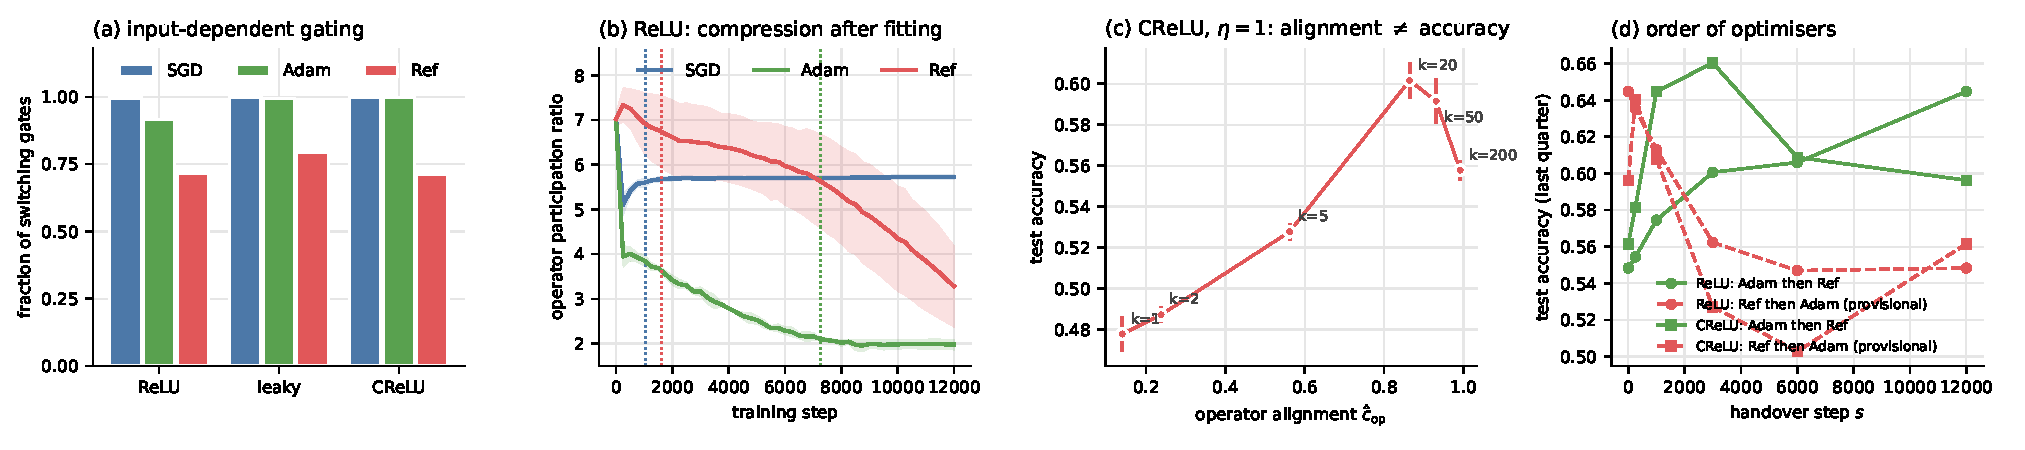
\includegraphics[width=\linewidth]{diagnostic_findings.pdf}
\caption{\zied{create one figure that explain all}Diagnosing different aspects of learning from reported table summaries. (a) A gate is switching when its state varies across $256$ probe inputs; lower fractions for \TOU\ persist with nonzero leaky-ReLU slopes. (b) ReLU operator participation ratios along the reported trajectory distinguish early fitting from later compression. (c) In the CReLU truncation sweep, increasing alignment does not monotonically increase test accuracy. (d) Both schedules allocate $6000$ updates to Adam and $6000$ to \TOU; their order changes the outcome. Panels reproduce Appendices~\ref{app:e8}, \ref{app:e9}, \ref{app:e7} and~\ref{app:e13}. Lines connect measured summaries; per-cell uncertainty and provenance checks remain in the blue notes. \nat{Drawn from the corrected cells ($k=50$, validation-selected). (b) mean $\pm$ s.d.\ over $5$ seeds of the $64$-input cheap probe, with dotted lines at each arm's mean fitting step. (c) bars are seed s.d. (d) last-quarter mean over $3$ seeds; the dashed Ref$\to$Adam curves are provisional because of the Adam handover defect.}}
\label{fig:diagnostic-findings}
\end{figure}

The gates link local operators to input-dependent computation. We measure the fraction of gates whose state changes across $256$ training inputs. In Figure~\ref{fig:diagnostic-findings}(a), this fraction under \TOU\ is \nat{$.715$} on ReLU, $.794$ on leaky ReLU and \nat{$.711$} on CReLU, compared with $.996$, $.999$ and $.999$ under SGD. \nat{(Corrected cells. Gate states come from the first saved snapshot at or after the anchor; snapshots are every $4000$ steps, so for \TOU\ this is step $4000$, about $2400$ steps after fitting. At the anchor itself, the cheap-probe gate diversity (the fraction of gates whose state differs between input $i$ and input $i+32$, averaged over the $32$ pairs of the $64$-input probe) orders the arms the same way: \TOU\ $.236/.272/.253$ against SGD $.425/.451/.388$ (ReLU/leaky/CReLU).)} The leaky-ReLU control is informative: both slopes are nonzero, yet $.107$ of its gates remain on the positive branch and $.099$ on the negative branch throughout the probe set. Reduced switching therefore describes more input-independent gating and cannot be identified simply with dead ReLU units. It complements the directional diagnosis by showing how the trained intervention changes the use of nonlinear features. The measurement concerns this finite input set, rather than all possible inputs.

\subsection{Operator compression can continue after fitting}

We measure pointwise operator complexity by the singular-value participation ratio
\begin{equation}
 \operatorname{PR}(P)=\frac{(\sum_j\sigma_j(P))^2}{\sum_j\sigma_j(P)^2},
 \label{eq:pr}
\end{equation}
averaged over $512$ inputs, excluding zero operators. Operator diversity is the participation ratio of the centred matrix of vectorised operators; it describes variation across inputs and has ceiling $\min(B-1,Cd)$. \nat{``Centred'' here means across inputs; class-centring, $(I-\mathbf1\mathbf1^\top/C)P(x)$, is a separate operation, reported in the red note below.}

Figure~\ref{fig:diagnostic-findings}(b) reveals a temporal distinction hidden by the final participation ratio. In the reported ReLU trajectory, \TOU's pointwise PR remains \nat{$6.62$} at step $2000$ and \nat{$6.37$} at step $4000$, while training loss has fallen to \nat{$2.1\cdot10^{-3}$ and $6.7\cdot10^{-7}$}. It then falls to \nat{$3.28$} at step $12000$. Thus the operator spectrum becomes much more concentrated after the network has already achieved a very small training loss. The first-post-threshold and final snapshot summaries tell the same qualitative story: PR changes from \nat{$6.38$ to $3.29$} and diversity from \nat{$191.5$ to $109.8$}, whereas SGD and Adam change little between their corresponding snapshots. \nat{(Corrected cell, $\eta=1$, $k=50$; the previous $7.30\to1.58$ came from $\eta=0.5$. \TOU\ does not rise above its initial PR of $7.02$ in the corrected cell. With an explicit criterion --- onset is the first probe at which PR falls one unit below its value at the anchor --- all $55$ fitting $k=50$ \TOU\ runs start the decline after fitting, with median lag $3250$ steps. Five of the six $k=200$ runs show no one-unit decline by step $12000$ (final PR $7.25$--$8.11$), and the sixth ends at $5.04$, against about $3$ at $k=50$. These runs fit later (steps $3250$--$5250$) but still have more post-fit time than the $k=50$ median lag, so the decline depends on truncation as well as on normalisation.)} Leaky ReLU shows a similar late decline; CReLU has a different initial ordering (Appendix~\ref{app:e9}).

This observation changes the interpretation of compression. A low participation ratio at the endpoint does not establish that comparable spectral concentration guided the preceding fit. Target normalisation provides a specific hypothesis: continued fixed-norm requests can reshape operators after the gradient becomes small. A raw-target ReLU control retains PR $6.27$ at step $12000$, versus $1.59$ for the normalised control. Its loss is also larger ($6.4\cdot10^{-4}$ versus $8\cdot10^{-11}$), so the comparison supports this hypothesis without isolating normalisation at matched progress. \nat{(This control was run against the $\eta=0.5$ cell, not the corrected $\eta=1$ cell, and is a single configuration whose run records have not been re-audited. The $k=200$ observation above is a second, independent route to the same question: $k=200$ runs are equally normalised, yet five of six do not decline.)} For classification, common-logit components can further change these statistics without changing predictions. \zied{Repeat the analysis on class-centred operators $(I-\mathbf1\mathbf1^\top/C)P(x)$; report zero-operator counts, snapshot offsets and seed uncertainty.}
\nat{Answer. Zero operators: none in any main cell (fraction $0.0000$ on every probe). Snapshot offsets: snapshots are every $4000$ steps, so the ``phase'' snapshot is step $4000$ for SGD and \TOU\ (anchors $1000$--$1750$) and $9600$ for ReLU Adam (anchor $7250$); the cheap-probe trajectory above is read at the anchor itself. Seed uncertainty: the corrected ReLU \TOU\ diversity is $191.5\pm33.5$. Class-centred operators: see Appendix~\ref{app:e9} (red table). \textbf{This changes the finding.} After centring, which removes the common-logit direction that softmax ignores, Ref's diversity does \emph{not} fall after fitting: it is $221.0\to218.8$ on ReLU, $220.2\to220.1$ on CReLU and $219.6\to216.7$ on leaky, the highest of the three arms in both windows. Its class-centred PR falls only from $6.5$--$6.7$ to $5.4$--$5.7$, against the raw $6.4$--$6.9\to1.8$--$3.3$. Most of the post-fitting ``compression'' therefore lies in a prediction-irrelevant direction. The section should be reframed as: after fitting, the normalised control keeps stepping mainly along the common-logit mode.}

\subsection{Interventions separate update geometry from learning outcomes}

A measuring direction becomes useful when it supports a testable intervention. We first vary how closely the trained control approximates it. For CReLU at target size $\eta=1$, all six $k\in\{1,2,5,20,50,200\}$ settings report training accuracy $1.000$. Estimated operator alignment rises from $.140$ to $.992$, while test accuracy rises from $.478$ to $.602$ at $k=20$ and then falls to $.558$ at $k=200$ (Figure~\ref{fig:diagnostic-findings}c). The sweep therefore separates closeness to the local reference from predictive success. The diagnostic tells us how the update changes; it does not prescribe the preferred amount of alignment. Each setting follows a different trajectory. \zied{figure: Verify this sweep's cell-level uncertainty and solver quality, and reconcile the original heatmap with the table before reuse (Appendix~\ref{app:e7}).}
\nat{Answer. The $\eta=1$ CReLU row is $3$ seeds per $k$ and $5$ at $k=50$; test s.d.\ is $.004$--$.011$ ($.478\pm.009$, $.487\pm.004$, $.528\pm.004$, $.602\pm.009$, $.592\pm.011$, $.558\pm.005$), and every probe passes $\mathrm{ne}<10^{-2}$. The current heatmap code reads the same cells at the same phase and gives the table's values; the $0.575/0.587$ come from an older endpoint version of the figure. Heatmap regeneration is still to do.}

We next ask whether an optimiser's effect depends on what has already been learned. Allocating $6000$ updates each to Adam and \TOU\ gives different outcomes when their order is reversed. Adam followed by \TOU\ gives accuracy $.606$ on ReLU and $.609$ on CReLU, compared with $.547$ and $.503$ for the reverse order (Figure~\ref{fig:diagnostic-findings}d). The allocation of update counts is the same, but the intermediate state and history differ. This order dependence motivates examining when gates and operator structure change, rather than attributing the final function only to the last optimiser used. It does not establish irreversibility under other schedules. \zied{Confirm evaluation windows, moment handling and paired-seed uncertainty for the switching study (Appendix~\ref{app:e13}).}
\nat{Answer. Window: last-quarter mean of test accuracy (steps $9000$--$12000$), three seeds, \TOU\ at $\eta=0.5$, $k=50$, Adam at $3\cdot10^{-3}$. Moment handling: \textbf{defect found}. At a \TOU$\to$Adam handover, Adam's $m$ and $v$ start at zero but its bias correction uses the global step, $1-\beta^{t+1}$ with $t$ the total step count. For handovers at $s\ge1000$ the correction is $\approx1$, so the first few hundred Adam steps are inflated, by $\approx3\times$ at the first step and up to $\approx6.5\times$ around the tenth. The \TOU$\to$Adam numbers ($.547$, $.503$) are therefore provisional until that half is re-run with the step count reset at handover. The Adam$\to$\TOU\ direction ($.606$, $.609$) is unaffected.}

The wider controls delimit this interpretation. Smoothing the control's \emph{weight increments} lowers alignment without reproducing Adam's advantage; because the step map changes over time, this is not momentum on realised operators (Appendix~\ref{app:e15}). Depth changes both learning and the accuracy of a fixed LSQR budget: at one depth-$32$ checkpoint, raising $k$ from $50$ to $3000$ changes alignment from $.71$ to $.9999$ (Appendix~\ref{app:e17}). Finally, the $49$-cell analysis reports within-architecture--optimiser correlations of $.41$ for alignment and $.91$ for gate diversity with test accuracy (Appendix~\ref{app:e18b}). \nat{(Pending recomputation: those $49$ cells include $4$ cells from the faulty K-FAC implementation, and the \TOU\ cells were pooled across $k$.)} These exploratory associations motivate joint analysis of update geometry and input-dependent structure; they do not identify a causal generalisation score.

\section{Related work}
\label{sec:related}

Deep linear models connect parameter dynamics with end-to-end learning. Exact dynamics for whitened quadratic regression with balanced, aligned initialisation \citep{saxe2014exact}, and the induced preconditioner under balanced gradient flow \citep{arora2018optimization}, explain how factorisation changes learning. Matrix-factorisation analyses investigate low-rank tendencies and the limits of norm-based implicit-bias descriptions \citep{gunasekar2017implicit,arora2019implicit,razin2020implicit,li2021towards}. Our framework builds on this operator perspective to diagnose a finite nonlinear training state. Fixed-gate Jacobian analysis studies depth scaling and spectral separation \citep{haas2026why}; conditional rank-bias results describe other structural effects \citep{timor2023implicit,jacot2023implicit}. We distinguish these state properties from the attainable motion and selected direction that produce their evolution.

The reference $-\eta(M^*M)^+\nabla_W\mathcal L$ connects the diagnosis to natural-gradient and Gauss--Newton geometry. In deep linear regression with whitened inputs and an isotropic quadratic output metric, the output-Jacobian Gram is proportional to the operator Gram, and Moore--Penrose representatives agree up to scale. Other generalised inverses can induce the same operator velocity with different parameter updates \citep{bernacchia2018exact}; cross-entropy does not inherit the isotropic-metric identity. Layerwise least-squares methods also use geometric reference steps to assess approximations \citep{dufortlabbe2026layerwise}. Here the reference supports measurements and interventions intended to interpret an optimiser's behaviour.

Minimum-perturbation analyses prescribe output changes on a batch, with exact single-layer expressions under appropriate assumptions and multilayer bounds \citep{evans2026theory}. Our target specifies complete local operators at sampled inputs. In the homogeneous setting, an output change constrains the action of an operator change along its input; the operator target constrains the full matrix. Jacobian-spectrum and dynamical-isometry studies \citep{wang2016extended,pennington2017resurrecting} motivate measuring the input--output map, while its parameter derivative $M$ is the object needed to diagnose reachability and update steering.

\section{Discussion and conclusion}
\label{sec:conclusion}

Operator projection makes three aspects of learning separately observable: what change the current network permits, how an optimiser steers that change, and which parameter motion is locally invisible. The experiments connect these questions to the use of gates, the timing of operator compression and the dependence on earlier optimisation. They show why predictive performance, instantaneous alignment and final operator complexity should be interpreted together. A diagnostic need not select the best optimiser to explain differences between their learning trajectories.

The present study concerns finite probe batches, local fixed-gate derivatives and explicit Euclidean metrics, mainly in small bias-free networks on MNIST-1D. Numerical certification matters at ill-conditioned checkpoints; the marked Adam estimates and aggregation conflicts remain unresolved. Incomplete CIFAR-10 runs and inconsistent cost records do not establish scalability. Within this scope, the framework provides a concrete route from comparing final predictors to investigating the functional changes through which optimisers learn them.

\clearpage
\subsection*{AI use statement}
For this revision, an AI assistant helped restructure and edit the prose, formulate and write mathematical arguments and proofs, review the methodology, interpret reported results, check selected references, draw a summary figure from reported table values, and prepare the LaTeX formatting. The assistant did not rerun the training experiments.
\zied{Confirm this disclosure and add any other AI assistance used in the research or manuscript. Record the disclosure in the submission form as well. The authors must verify the scientific content, references and results before submission.}
\nat{Correction: the last sentence of the statement is false for this project. An AI coding assistant (Claude) also wrote and debugged most of the experiment and analysis code, launched and monitored the training runs, computed the reported tables and figures, and audited the implementation, including finding the K-FAC scaling fault, the cold-state kernel measurement, the cell-pooling selection bug and the Adam handover defect. The disclosure should say so.}

\subsection*{Ethics statement}
This work studies how optimisation rules change the functions computed by neural networks. Its direct contribution is a diagnostic framework and a small-scale empirical analysis. The measurements do not provide guarantees of model reliability, fairness or robustness, and should not be used as substitutes for evaluating those properties in a deployment setting.

\subsection*{Reproducibility statement}
The operator definitions and proofs are given in Sections~\ref{sec:method}--\ref{sec:numerics} and Appendices~\ref{app:theory}--\ref{app:solver}. Appendix~\ref{app:protocol} records the experimental settings and unresolved details required to reproduce the reported results.
\zied{Supply an anonymised implementation, the run manifest and checkpoints, and resolve the marked numerical and protocol checks before claiming reproducibility.}
\nat{Status: every run directory stores \texttt{config.json}, \texttt{meta.json} (git SHA, device, torch version), \texttt{metrics.jsonl}, a checkpoint and weight snapshots every $4000$ steps ($5.6$\,GB in total). An anonymised code release and a per-table manifest are still to do.}

\bibliography{references}
\bibliographystyle{iclr2027_conference}
\clearpage
\appendix
\raggedbottom

\section{Operator geometry and proofs}
\label{app:theory}

\subsection{The operator and its local derivative}

For each input $x_i$, let $h_0=x_i$, $z_\ell=W_\ell h_{\ell-1}$ and
$h_\ell=D_\ell(z_\ell)z_\ell$ for $\ell<L$, with a linear output layer.
Writing the gates explicitly gives
\begin{equation}
 P_i=W_LD_{L-1}(x_i)W_{L-1}\cdots D_1(x_i)W_1,
 \qquad f_W(x_i)=P_i x_i.
 \label{eq:app-operator}
\end{equation}
For ReLU, leaky ReLU and CReLU, this identity follows coordinate by coordinate from the definition of the activation. Where the network is differentiable with respect to its input, $P_i=\partial f_W(x_i)/\partial x_i$. At a zero pre-activation, a gate convention still gives the factorisation in Equation~\eqref{eq:app-operator}, but the ordinary input Jacobian need not exist.

The dimensions of a gate need not be square. If $z\in\mathbb R^d$, CReLU has
\begin{equation}
 D(z)=\begin{bmatrix}
 \operatorname{diag}(\mathbf 1[z>0])\\
 -\operatorname{diag}(\mathbf 1[z<0])
 \end{bmatrix}\in\mathbb R^{2d\times d}.
\end{equation}
The next weight matrix therefore has $2d$ input columns. For this strict-sign convention, $D(z)^\top D(z)=I$ only when every coordinate of $z$ is nonzero; in general it equals $\operatorname{diag}(\mathbf 1[z\ne0])$. If the next weight matrix is $[O\mid-O]$, its action on the CReLU activations is nevertheless $Oz$ for every $z$, including coordinates equal to zero. Away from zero pre-activations, $[O\mid-O]D(z)=O$. A chain built from such paired blocks represents the corresponding linear product at initialisation. It is an orthogonal operator only when that product is square and orthogonal; rectangular input and output layers require their own rank and conditioning assumptions.

Define the contexts, with input dependence understood, by
\begin{equation}
 \begin{aligned}
 B_{1,i}&=I,& B_{\ell+1,i}&=D_\ell(x_i)W_\ell B_{\ell,i},\\
 A_{L,i}&=I,& A_{\ell,i}&=A_{\ell+1,i}W_{\ell+1}D_\ell(x_i).
 \end{aligned}
\end{equation}
Then $P_i=A_{\ell,i}W_\ell B_{\ell,i}$ for every layer, with compatible dimensions also for CReLU.

Suppose that all pre-activations on the finite probe batch are nonzero. By continuity, there is a neighbourhood of $W$ on which all of those gate signs remain fixed. In that neighbourhood, $P_i$ is a polynomial in the weights. Expanding the product gives
\begin{equation}
 P_i(W+d)-P_i(W)
 =\sum_{\ell=1}^L A_{\ell,i}d_\ell B_{\ell,i}
   +O(\|d\|_{\mathcal W}^2).
 \label{eq:app-local}
\end{equation}
The linear term is the step map of Equation~\eqref{eq:stepmap}. The bound is local to this fixed-gate neighbourhood. It does not cover a finite step that crosses an activation boundary: the network output is continuous there, but its input Jacobian, and hence the operator $P_i$, can jump. At a boundary, the frozen-gate map is an explicitly chosen local model rather than a generally valid derivative of $W\mapsto P_i(W)$.

\subsection{Batch geometry and the adjoint}

Let $\mathcal W$ be the product of the layer matrix spaces, with
$\langle d,e\rangle_{\mathcal W}=\sum_\ell\operatorname{tr}(d_\ell^\top e_\ell)$.
For a batch of $B$ inputs, the operator space is
$\mathcal H=(\mathbb R^{C\times d})^B$, equipped with
\begin{equation}
 \langle H,K\rangle_{\mathcal H}
 =\frac1B\sum_{i=1}^B\operatorname{tr}(H_i^\top K_i).
 \label{eq:app-inner}
\end{equation}
The trace identity
$\langle A d B,H\rangle_F=\langle d,A^\top H B^\top\rangle_F$
then gives
\begin{equation}
 (M^*H)_\ell
 =\frac1B\sum_{i=1}^B A_{\ell,i}^\top H_i B_{\ell,i}^\top.
 \label{eq:app-adjoint}
\end{equation}
Here $M^*$ denotes the adjoint for these two inner products. This convention keeps the batch-average loss and its gradient consistent.

In particular, for
$\mathcal L(W)=B^{-1}\sum_i\ell(f_W(x_i),y_i)$, put
$g_i=\nabla_f\ell(f_W(x_i),y_i)$ and $G_i=g_i x_i^\top$.
Then $\nabla_W\mathcal L=M^*G$ wherever the preceding derivative is valid. Squared loss means $\ell(f,y)=\tfrac12\|f-y\|^2$, for which $g_i=f_W(x_i)-y_i$; for softmax cross-entropy, $g_i=\operatorname{softmax}(f_W(x_i))-e_{y_i}$. Thus the gradient-descent update with step size $\eta$ is exactly $M^*b$ for the target $b=-\eta G$. This identity requires the update and the diagnostic to use the same batch and loss reduction.

\subsection{The reference and the decomposition}

All statements in this subsection are finite-dimensional and hold for an arbitrary linear step map $M$. Let $b$ be the target in Equation~\eqref{eq:target}, and let $\Pi=MM^+$ be the orthogonal projector in $\mathcal H$ onto $\operatorname{range}(M)$. If
\begin{equation}
 Mv_j=\sigma_j u_j,\qquad M^*u_j=\sigma_j v_j,\qquad \sigma_j>0,
\end{equation}
is a singular system in the specified inner products, then
\begin{equation}
 r:=\Pi b=\sum_j\langle b,u_j\rangle_{\mathcal H}u_j,
 \quad
 d_{\mathrm{ref}}=M^+b
 =\sum_j\frac{\langle b,u_j\rangle_{\mathcal H}}{\sigma_j}v_j.
 \label{eq:app-svd-ref}
\end{equation}
Every $d$ with $Md=r$ has the form $d=d_{\mathrm{ref}}+z$, where $z\in\ker M$. Since $d_{\mathrm{ref}}\in\operatorname{range}(M^*)=(\ker M)^\perp$,
\begin{equation}
 \|d\|_{\mathcal W}^2=\|d_{\mathrm{ref}}\|_{\mathcal W}^2+\|z\|_{\mathcal W}^2.
\end{equation}
This proves that Equation~\eqref{eq:reference} is the unique minimum-norm least-squares solution. It also gives
$M^+=(M^*M)^+M^*=M^*(MM^*)^+$, and hence the preconditioned-gradient expression.

To prove Proposition~\ref{prop:decomposition}, write $b=r+b_\perp$, where $b_\perp\perp\operatorname{range}(M)$. For every update $d$,
\begin{equation}
 \|Md-b\|_{\mathcal H}^2
 =\|b_\perp\|_{\mathcal H}^2+\|Md-r\|_{\mathcal H}^2.
 \label{eq:app-pythagoras}
\end{equation}
The first term is the unavoidable residual of this local model; the second is the discrepancy between the candidate operator change and the projection. If $b$, $r$ and $Md$ are nonzero, orthogonality also yields
\begin{equation}
 \cos_{\mathcal H}(Md,b)
 =\frac{\|r\|_{\mathcal H}}{\|b\|_{\mathcal H}}
    \cos_{\mathcal H}(Md,r)
 =\alpha\cos_{\mathrm{op}}.
 \label{eq:app-angle}
\end{equation}
The same identity explains which information the instantaneous loss slope aggregates. At a differentiable state, for the same batch, loss and metrics as above, $\nabla_W\mathcal L=M^*G$ and $b=-\eta G$ imply
\begin{equation}
 \begin{aligned}
 D\mathcal L(W)[u]
 &=\langle G,Mu\rangle_{\mathcal H}
 =-\frac{\langle b,Mu\rangle_{\mathcal H}}{\eta}\\
 &=-\frac{\|b\|_{\mathcal H}\|Mu\|_{\mathcal H}}{\eta}
       \alpha c_{\rm op}.
 \end{aligned}
 \label{eq:app-loss-slope}
\end{equation}
The last expression requires the diagnostic cosines to be defined. It separates the magnitude of the operator change, target reachability and alignment within the reachable space, whereas the loss derivative reports only their product. It is an instantaneous, local identity; by itself it gives no guarantee about a finite training step, particularly one crossing activation boundaries. A kernel component contributes zero to this derivative, but can affect higher-order changes and subsequent states.

Consequently, $\alpha$ is the greatest alignment with $b$ attainable by a nonzero vector in $\operatorname{range}(M)$ when $r\ne0$. It is a fraction of the target norm, not an upper bound on the norm of an arbitrary induced update: multiplying $d$ by a scalar can make $\|Md\|$ arbitrarily large. If $b=0$, $r=0$, $Md=0$, or $d_{\mathrm{ref}}=0$, any ratio or cosine with a zero denominator is undefined and must be reported as such.

For a weight update, its orthogonal decomposition is
\begin{equation}
 d=M^+Md+(I-M^+M)d,
 \quad
 M^+Md\in\operatorname{range}(M^*),
 \quad
 (I-M^+M)d\in\ker M.
 \label{eq:app-kernel}
\end{equation}
Thus a kernel fraction defined by
$\|(I-M^+M)d\|_{\mathcal W}/\|d\|_{\mathcal W}$
is a norm fraction; its square is the fraction of squared norm. A zero operator derivative on the probe batch establishes first-order invariance on that batch. It does not establish invariance for finite steps or for unseen inputs, and the batch kernel need not consist solely of parameter symmetries.

For a candidate $u$, write $u_R=M^+Mu$, $u_K=(I-M^+M)u$ and $u_{\rm ref}=M^+b$. If $u$, $u_R$ and $u_{\rm ref}$ are nonzero, its weight cosine and kernel fraction satisfy
\begin{equation}
 c_{\rm w}=\sqrt{1-q^2}\,
     \cos_{\mathcal W}(u_R,u_{\rm ref}),
 \qquad q=\frac{\|u_K\|_{\mathcal W}}{\|u\|_{\mathcal W}}.
 \label{eq:app-weight-cosine}
\end{equation}
Indeed, $u_K\perp u_{\rm ref}$, so the numerator of $c_{\rm w}$ is $\langle u_R,u_{\rm ref}\rangle_{\mathcal W}$, while Pythagoras gives $\|u_R\|_{\mathcal W}/\|u\|_{\mathcal W}=\sqrt{1-q^2}$. A small weight cosine can therefore reflect a different direction within $\operatorname{range}(M^*)$, motion in $\ker M$, or both. It does not identify kernel motion on its own. If $u_R=0$ but $u$ and $u_{\rm ref}$ are nonzero, then $q=1$ and $c_{\rm w}=0$ directly; the cosine involving $u_R$ is undefined and Equation~\eqref{eq:app-weight-cosine} is not used.

\subsection{An example of what the diagnostics distinguish}
\label{app:diagnostic-example}

Consider the local map and target
\begin{equation}
 M(u_1,u_2,u_3)=(u_1,2u_2,0),\qquad b=(1,1,1),
 \label{eq:app-example-map}
\end{equation}
with Euclidean inner products. This is an analytic illustration, not a training experiment. The third target component is unreachable, the second reachable parameter direction is amplified twice as strongly as the first, and the third parameter direction lies in the kernel. Direct calculation gives
\begin{equation}
 r=\Pi b=(1,1,0),\qquad
 \alpha=\sqrt{\frac23},\qquad
 u_{\rm ref}=M^+b=(1,\tfrac12,0).
\end{equation}

Suppose the operator-space loss gradient at the current state is $G=-b$. This occurs, for example, for the quadratic loss $\tfrac12\|P-P_\star\|^2$ at $P_\star=P+b$. The negative parameter gradient is $M^*b=(1,2,0)$. Table~\ref{tab:app-example} compares the reference, a positively rescaled gradient direction, and the reference with an added kernel component. Every row satisfies $\langle b,Mu\rangle=2$. Consequently, an infinitesimal parameter step $\varepsilon u$ has the same first-order loss change in all three cases,
\begin{equation}
 \mathcal L(W+\varepsilon u)-\mathcal L(W)
 =-2\varepsilon+O(\varepsilon^2),
 \label{eq:app-example-loss}
\end{equation}
when the local smoothness assumptions hold. Rescaling the target to $\varepsilon b$ also rescales its reference to $\varepsilon u_{\rm ref}$; all the displayed diagnostic scores remain unchanged.

\begin{table}[t]
\centering\small
\caption{Three update directions with the same first-order loss decrease in the analytic example. Their operator changes and parameter routes differ.}
\label{tab:app-example}
\begin{tabular}{lccccc}
\toprule
Update & $u$ & $Mu$ & $c_{\rm op}$ & $c_{\rm w}$ & $q$\\
\midrule
Reference & $(1,\tfrac12,0)$ & $(1,1,0)$ & $1$ & $1$ & $0$\\
Rescaled gradient & $(\tfrac25,\tfrac45,0)$ & $(\tfrac25,\tfrac85,0)$
 & $5/\sqrt{34}$ & $4/5$ & $0$\\
Reference + kernel & $(1,\tfrac12,\tfrac{\sqrt5}{2})$ & $(1,1,0)$
 & $1$ & $1/\sqrt2$ & $1/\sqrt2$\\
\bottomrule
\end{tabular}
\end{table}

The gradient direction assigns four times as much operator motion to the second coordinate as to the first. Its parameter update has no kernel component, so this redistribution cannot be attributed to locally invisible motion. The third row instead has the same operator change as the reference, with half of its squared parameter norm in the kernel. Its smaller weight cosine comes entirely from that added component, as Equation~\eqref{eq:app-weight-cosine} shows. Finally, all three share the same reachability $\alpha$: no choice of update can supply the third requested component through this local map. A scalar first-order loss change does not distinguish these three explanations.

The example can be realised by a small factored linear model. Let $f_{a,b,c,d}(x)=abx_1+cdx_2$ for $x\in\mathbb R^3$, with no dependence on $x_3$, and consider $a=b=1/\sqrt2$, $c=d=\sqrt2$. Use the orthonormal increment coordinates
\begin{equation}
 \begin{aligned}
 u_1&=(\delta a+\delta b)/\sqrt2,&
 u_2&=(\delta c+\delta d)/\sqrt2,\\
 u_3&=(\delta a-\delta b)/\sqrt2,&
 u_4&=(\delta c-\delta d)/\sqrt2.
 \end{aligned}
\end{equation}
The operator is $P=(ab,cd,0)$, and its derivative is $(u_1,2u_2,0)$. Setting the additional kernel coordinate $u_4=0$ yields Equation~\eqref{eq:app-example-map}, without changing the Euclidean norm. This construction also illustrates the local qualification: a pure $u_3=t$ perturbation changes $ab$ by $-t^2/2$ even though its first-order operator change is zero. Kernel motion is not generally finite-step function preservation.

\subsection{What is invariant}

At fixed weights, batch and optimiser state, both diagnostic cosines are invariant under multiplication of the candidate update by a positive scalar. They are also invariant under positive rescaling of $b$, which rescales $r$ and $d_{\mathrm{ref}}$. This removes the current scalar step length from the directional comparison. It does not remove the effect of a learning-rate history on the weights, gates or optimiser state, nor does it make a finite-step trajectory independent of step size.

The reference depends on two declared metrics: the Frobenius metric on the sampled operators and the Euclidean metric on the weights. Under a smooth invertible change of weight coordinates $W=\phi(\theta)$, the derivative becomes $M\,D\phi$. Its range is unchanged, so the projected operator direction remains the same when the operator metric is held fixed. Its minimum-Euclidean-norm lift generally changes. For example, with a scalar output operator $P=w_1+w_2$, the minimum-norm lift of a change $b$ is $(b/2,b/2)$. In coordinates $w_1=c\theta_1$, $w_2=\theta_2$, minimum Euclidean norm in $\theta$ gives the weight displacement $(c^2b/(c^2+1),b/(c^2+1))$. The two lifts have the same operator effect but different weight directions. Changing input coordinates can also change the Frobenius operator metric. The reference is therefore well defined relative to these choices; it is not a metric-free notion of an unbiased update.

\section{Deep linear networks}
\label{app:linear}

For a deep linear chain, $P=W_L\cdots W_1$ is shared by the batch. Its loss gradient is the aggregate matrix
\begin{equation}
 \overline G=\frac1B\sum_{i=1}^B g_i x_i^\top.
\end{equation}
In this subsection the output of the step map is a single matrix, with its ordinary Frobenius inner product:
\begin{equation}
 \mathcal M(d)=\sum_\ell A_\ell d_\ell B_\ell,
 \qquad
 (\mathcal M^*H)_\ell=A_\ell^\top H B_\ell^\top.
\end{equation}
The shared target is $b_{\mathrm{lin}}=-\eta\overline G$. This reduction has the same minimum-norm least-squares weight update as stacking per-example targets, because
\begin{equation}
 \frac1B\sum_i\|\mathcal M(d)+\eta G_i\|_F^2
 =\|\mathcal M(d)+\eta\overline G\|_F^2
   +\frac{\eta^2}{B}\sum_i\|G_i-\overline G\|_F^2.
\end{equation}
However, the two target spaces have different reachability denominators. Reachability of the shared target must not be identified with reachability of the full collection of per-example targets.

Define the self-adjoint positive-semidefinite transfer operator
\begin{equation}
 \mathcal T(H)=\mathcal M\mathcal M^*(H)
 =\sum_\ell A_\ell A_\ell^\top H B_\ell^\top B_\ell.
 \label{eq:app-transfer}
\end{equation}
The exact solution of the \emph{linearised} reference problem is
\begin{equation}
 H=\mathcal T^+b_{\mathrm{lin}},\qquad
 (d_{\mathrm{ref}})_\ell=A_\ell^\top H B_\ell^\top,
 \qquad
 \mathcal M(d_{\mathrm{ref}})=\mathcal T\mathcal T^+b_{\mathrm{lin}}.
 \label{eq:app-linear-reference}
\end{equation}
This follows directly from $\mathcal M^+=\mathcal M^*(\mathcal M\mathcal M^*)^+$. It is an exact algebraic characterisation at arbitrary weights; evaluating $\mathcal T^+$ can still require a numerical linear solve. It is not a closed-form solution of the finite product constraint $\prod_\ell(W_\ell+d_\ell)=P+b_{\mathrm{lin}}$.

A sufficient condition for $\mathcal M$ to be surjective is that, for some layer $\ell$, $A_\ell$ has full row rank and $B_\ell$ has full column rank. Given any matrix $H$, the single-layer update $d_\ell=A_\ell^+ H B_\ell^+$ then satisfies $A_\ell d_\ell B_\ell=H$. This condition holds, for example, for a square chain with invertible factors. A parameter count alone does not imply it. If two or more layers are zero, all first derivatives of the product can vanish even when the network has many parameters. In a gated model, two probe inputs with the same gate pattern necessarily have the same operator and the same frozen-gate operator derivative, which already excludes arbitrary independent targets at those inputs.

For a linear chain, the output Jacobian maps $d$ to $(\mathcal M(d)x_i)_i$. Its Gram satisfies
\begin{equation}
 J_f^*J_f(d)=\mathcal M^*\big(\mathcal M(d)C_x\big),
 \qquad C_x=\frac1B\sum_i x_i x_i^\top.
\end{equation}
Thus $C_x=cI$, $c>0$, makes the output Gram proportional to the operator Gram. For squared loss, or an isotropic Gaussian observation model with fixed variance, this connects the reference to Gauss--Newton or natural gradient, up to a scalar step size. For softmax cross-entropy, the Fisher contains an additional output metric depending on class probabilities, so whitening the inputs alone does not establish the same identity.

\subsection{Conservation under continuous flow}

Consider the DLN flow $\dot W_\ell=A_\ell^\top\Lambda B_\ell^\top$, where the same matrix $\Lambda$ is used for every layer and may depend on time. The context recursions imply
\begin{equation}
 W_{\ell+1}^\top\dot W_{\ell+1}=\dot W_\ell W_\ell^\top,
 \qquad
 \dot W_{\ell+1}^\top W_{\ell+1}=W_\ell\dot W_\ell^\top.
\end{equation}
Adding these identities proves
\begin{equation}
 \frac{\mathrm d}{\mathrm dt}
 \big(W_{\ell+1}^\top W_{\ell+1}-W_\ell W_\ell^\top\big)=0.
 \label{eq:app-conservation}
\end{equation}
Gradient flow and the exact reference vector field are of this form. This does not imply exact conservation for discrete gradient descent or a discrete reference update. If $d_\ell=A_\ell^\top\Lambda B_\ell^\top$, direct expansion gives the exact finite-step identity
\begin{equation}
 \begin{split}
 &(W_{\ell+1}+d_{\ell+1})^\top(W_{\ell+1}+d_{\ell+1})
 -(W_\ell+d_\ell)(W_\ell+d_\ell)^\top\\
 &\quad-\big(W_{\ell+1}^\top W_{\ell+1}-W_\ell W_\ell^\top\big)
 =d_{\ell+1}^\top d_{\ell+1}-d_\ell d_\ell^\top.
 \end{split}
 \label{eq:app-discrete-conservation}
\end{equation}
The drift is second order in the update and is generally nonzero.

For generic ReLU or leaky-ReLU networks, arbitrary changes of hidden basis do not preserve the function. Positive rescaling of an individual hidden unit does: multiply its incoming row $a$ by $c>0$ and divide its outgoing column $b$ by $c$. The symmetry tangent is $(a,-b)$ and lies in $\ker M$ at differentiable points. A flow in $\operatorname{range}(M^*)$ is orthogonal to it, giving $\langle a,\dot a\rangle=\langle b,\dot b\rangle$ and conservation of $\|a\|^2-\|b\|^2$. This per-unit statement does not justify conservation of the full matrix imbalance in Equation~\eqref{eq:app-conservation} for generic gated networks.

Finally, at the all-zero DLN parameter point and depth $L\ge2$, $\mathcal M=0$ and the reference is zero. A nonzero finite factorisation of a target matrix can exist there, but finding it solves a different, nonlinear constraint problem. The least-squares reference does not escape points where its own derivative vanishes.

\section{Numerical approximation and certification}
\label{app:solver}

\subsection{Truncation and damping}

In exact arithmetic, zero-initialised LSQR searches a nested sequence of Krylov spaces
\begin{equation}
 \mathcal K_k=\operatorname{span}\{M^*b,(M^*M)M^*b,\ldots,(M^*M)^{k-1}M^*b\}
 \subseteq\operatorname{range}(M^*).
\end{equation}
Its first nonzero iterate is a positive multiple of $M^*b$, so it has the gradient-descent direction. Its scalar coefficient is selected by the least-squares problem; a normalised-target, one-iteration training rule is therefore not ordinary gradient descent with a fixed learning rate. At a fixed $M$ and $b$, the undamped least-squares residual cannot increase with $k$. If $d_k$ is the exact minimiser on $\mathcal K_k$, $Md_k$ is the orthogonal projection of $b$ onto $M\mathcal K_k$, and
$\cos(Md_k,r)=\|Md_k\|/\|r\|$ when these vectors are nonzero. The resulting monotonicity is a fixed-problem statement. It does not imply monotonic diagnostic values across separately trained runs with different $k$.

With the convention in Equation~\eqref{eq:damped}, damping solves
\begin{equation}
 d_\lambda=\arg\min_d\left\{\|Md-b\|_{\mathcal H}^2+\lambda\|d\|_{\mathcal W}^2\right\},
 \qquad\lambda>0.
\end{equation}
The unique solution and its operator effect are
\begin{equation}
 \begin{split}
 d_\lambda&=(M^*M+\lambda I)^{-1}M^*b,\\
 Md_\lambda&=\sum_j\frac{\sigma_j^2}{\sigma_j^2+\lambda}
                 \langle b,u_j\rangle_{\mathcal H}u_j.
 \end{split}
 \label{eq:app-damped}
\end{equation}
The second expression is a filtered target, not an orthogonal projection. It approaches $r$ as $\lambda\downarrow0$ for a fixed finite-dimensional problem. Its norm is no greater than $\|r\|$, but its direction can differ when singular values have different damping factors. Treating a damped solution as the exact reference requires a check that the quantities being reported are insensitive to the chosen damping.

\subsection{What residuals establish}

The undamped normal-equation residual is
$r_N=M^*(Md-b)$. It measures least-squares stationarity. For the damped problem, the relevant residual is instead
$r_\lambda=M^*(Md-b)+\lambda d$; the exact damped solution has $r_\lambda=0$ and $r_N=-\lambda d_\lambda$. Reporting both distinguishes failure to solve the regularised system from the effect of regularisation itself.

Neither the plain residual nor $r_N$ detects an added exact kernel component. With $M=[1\;0]$, $b=1$ and $d=(1,t)$, both residuals are zero for every $t$, although only $t=0$ gives the minimum-norm solution. Retaining the iterate with smallest normal residual therefore cannot by itself certify minimum norm. Damping penalises such a component, while an explicit small-instance singular-value decomposition can check the minimum-norm property directly.

A small relative normal residual also need not imply a small operator error when the nonzero singular values are poorly conditioned. For example, take $M=\operatorname{diag}(1,\varepsilon)$, $b=(1,1)$ and $d=(1,0)$. The relative normal residual is $\varepsilon/\sqrt{1+\varepsilon^2}$, which tends to zero, but $\|Md-\Pi b\|=1$. A tolerance on $r_N$ is consequently an operational quality check, not a condition-independent error guarantee for reachability, weight angles or kernel fractions.

An approximate vector $y=Md$ still supplies rigorous lower bounds on reachability without identifying it with $r$. In exact arithmetic,
\begin{equation}
 \alpha\ge
 \sqrt{\max\left\{0,1-\frac{\|b-y\|_{\mathcal H}^2}{\|b\|_{\mathcal H}^2}\right\}},
 \qquad
 \alpha\ge\frac{|\langle b,y\rangle_{\mathcal H}|}
                   {\|b\|_{\mathcal H}\|y\|_{\mathcal H}}
 \label{eq:app-reach-bound}
\end{equation}
whenever the displayed denominators are nonzero. The first bound uses optimality of the projection residual; the second uses $y\in\operatorname{range}(M)$ and Cauchy--Schwarz. By contrast, $\|y\|/\|b\|$ is not a lower bound for an arbitrary unconverged numerical iterate. It has that interpretation for an exact restricted least-squares projection, or for the exact damped filter above, under their respective assumptions.

Numerical verification must therefore separate the adjoint identity, least-squares stationarity, minimum-norm behaviour and finite-step fidelity. They are different properties. In particular, calibrating zero kernel fractions for gradient descent at one set of checkpoints does not certify a projection at another optimiser's checkpoints, whose step map can have a different spectrum. Finite-step fidelity additionally requires evaluating the actual difference $(P_i(W+d)-P_i(W))_i$ and comparing it with $Md$, because no linear-system residual measures gate changes.

\paragraph{\nat{Checks run for this revision.}}
\nat{\emph{SVD agreement.} On small gated networks (width $10$, depth $4$, $6$ inputs, $360$--$600$ parameters), with $M$ formed densely and $M^+b$ from its SVD, the damped LSQR solve ($5000$ iterations, $\lambda_{\rm rel}=10^{-7}$) matches to relative error $1.3\cdot10^{-4}$ (ReLU), $4.7\cdot10^{-5}$ (CReLU) and $1.2\cdot10^{-4}$ (leaky, one draw). On a second leaky draw, whose smallest nonzero singular value is $1.8\cdot10^{-5}\sigma_{\max}$, the solve is within $2.6\%$ in operator space but $65\%$ off in weight space, because $\|M^+b\|$ is dominated by those small singular directions. Operator-space quantities ($\alpha$, $c_{\rm op}$) are therefore much more robust to ill-conditioning than weight-space ones ($c_{\rm w}$, $\|u^{\rm ref}\|$), which is exactly the failure mode described above. The kernel component of the damped solution is at most $1.3\cdot10^{-4}$ of its norm.}

\nat{\emph{Finite-step fidelity.} At the convergence-phase checkpoint of the corrected \TOU\ cell, one actual training step ($\|\Delta W\|/\|W\|\approx5\cdot10^{-3}$) flips at least one gate on $63$ of $64$ probe inputs (ReLU) and $64$ of $64$ (CReLU). The realised operator change is $24\times$ (ReLU) and $18\times$ (CReLU) larger than the first-order prediction $Md$ in relative error. On the one ReLU input without a flip, the linear prediction is accurate to $1.6\%$. For SGD at its trained checkpoint, a much smaller step ($\approx2\cdot10^{-5}$) still flips gates on $4$ of $64$ (ReLU) and $16$ of $64$ (CReLU) inputs, and those jumps again dominate the realised change ($\approx150\times$). On random-initialisation networks, where no gate flips, the error scales as $O(t)$ as it should. Consequently the realised finite-step operator motion at trained states is dominated by gate crossings for every rule tested, and $c_{\rm op}$, $\alpha$ and $q$ describe the local derivative only. This strengthens the local-only reading used in the main text and should be stated there.}


%%%%%%%%%%%%%%%%%%%%%%%%%%%%%%%%%%%%%%%%%%%%%%%%%%


\section{Experimental protocol and supporting results}\label{app:protocol}

The supplement records the experiments used to diagnose optimiser behaviour, including settings that did not reach the fitting threshold. We distinguish the exact reference $M^+b$ from the \emph{reference-following control} (Ref) used in training. Ref uses $k=50$ LSQR iterations unless a sweep specifies otherwise and normalises its target. The figures supplied with the draft call this arm ``reference'' or ``operator''. The minibatch baseline is called SGD here; the original draft calls it ``gradient descent''. For the linear experiment we retain the original name gradient descent; its batch protocol needs to be specified.

These results have been checked for internal consistency, but the supplied package contains neither the experiment code nor the run records needed to recompute them. Tables below preserve reported values; blue notes identify numerical conflicts, missing protocol details and incomplete comparisons. The main paper uses these records to examine update steering, input-dependent gating, the timing of compression and the effect of optimiser history (Sections~\ref{sec:experiments} and~\ref{sec:diagnostics}). These diagnostic questions organise the interpretation; the checks below delimit what the supplied observations establish.

\paragraph{Data and training.}
The main task is MNIST-1D \citep{greydanus2020mnist1d}, with input dimension $40$, $10$ classes, and reported splits of \nat{$3000$} training, $1000$ validation and $1000$ test examples. Training uses cross-entropy, minibatches of $100$, a bias-free network of depth $8$ and width $128$, and He initialisation. ReLU and CReLU form the main comparison; leaky ReLU uses slope $0.1$. The budget is $12000$ updates. The main comparison uses five seeds for ReLU and CReLU and three for leaky ReLU; sweeps use their separately stated counts. Reported uncertainties are standard deviations across seeds unless stated otherwise.

\zied{Supply the MNIST-1D generation version, data seed, split construction, preprocessing and split hashes. The reported 4000/1000/1000 split needs an explicit generation or resampling procedure. Specify whether width 128 counts pre-activation units or post-CReLU features, all layer shapes, initialisation gains, training precision, minibatch sampling and shuffle seeds. Release the configuration and checkpoint manifest that links each table to its runs.}
\nat{Answer. Generator: \texttt{mnist1d} 0.0.2.post1, \texttt{make\_dataset} with default arguments (5000 samples, train split $0.8$, template length $12$, padding $[36,60]$, max translation $48$, correlated noise $0.25$, i.i.d.\ noise $0.02$, shear $0.75$, length $40$) and \emph{data seed equal to the run seed}. Each seed therefore regenerates the dataset, including the test set, so seed standard deviations include data variation. Split: a seeded permutation of the $4000$ generator-train points gives $1000$ validation and the remaining $3000$ training points; the test set is the generator's $1000$ test points. Preprocessing: one scalar mean and standard deviation from the training split. Width $128$ counts pre-activation units; CReLU layers therefore have $256$ inputs. Shapes: $W_1\in\R^{128\times40}$, $W_{2..7}\in\R^{128\times128}$ ($128\times256$ for CReLU), $W_8\in\R^{10\times128}$ ($10\times256$). Initialisation: $\mathcal N(0,2/\text{fan-in})$ with fan-in the post-activation width. Training: float32; minibatches are drawn with replacement by a generator seeded with the run seed; probes run in float64. Split hashes and a per-table manifest are still to do.}

\paragraph{Target and optimiser settings.}
The training arm supplies $(-\eta G(x)/\|G\|)_x$ to LSQR; diagnostics use the unnormalised target. This distinguishes a normalised, truncated algorithm from the exact reference. Normalising the target does not guarantee a constant weight-step norm or a constant realised operator-step norm: reachability, solver truncation and the current step map also enter. The selected settings in the principal comparison are SGD $0.1$, Adam $0.003$, Ref $0.5$ on ReLU; SGD $0.03$, Adam $0.003$, Ref $10$ on CReLU; and SGD $0.1$, Adam $0.003$, Ref $1$ on leaky ReLU.

\nat{Correction to the sentence above: the training arm feeds LSQR $b_i=-\eta(g_i/\|g\|_F)x_i^\top$, where $\|g\|_F$ is the Frobenius norm of the whole batch of output residuals, guarded by $\max(\cdot,10^{-12})$.}
\zied{Define whether the normaliser is a norm of the whole batch, a per-example norm or another residual, and state its zero-residual guard. Give every learning-rate and target-size grid, optimiser coefficients and epsilon values, schedules, weight decay, clipping, solver initialisation and stopping rules. A target-size grid is still hyperparameter tuning; remove claims that Ref has no parameter to tune.}
\nat{Answer. Whole-batch norm of the output residual, guard $10^{-12}$ (above). Grids at depth $8$, width $128$: SGD $\{0.003,0.01,0.03,0.1\}$ (CReLU without $0.1$, so its selected $0.03$ is at the edge of its grid), Adam $\{10^{-3},3\cdot10^{-3},10^{-2},3\cdot10^{-2}\}$ ($\beta=(0.9,0.999)$, $\epsilon=10^{-8}$), \TOU\ $\eta\in\{0.1,0.3,0.5,1\}$ at $k=50$ (plus the E7 sweep). No schedules, weight decay or clipping. LSQR starts from zero, runs exactly $k$ iterations (no early stopping, $\mathrm{atol}=0$), and raises an error if $\|d\|>10^6\|b\|$ (drift into $\ker M$). Agreed on tuning: $\eta$ is a tuned hyperparameter.}

\paragraph{Measurement phase and selection.}
The reported convergence phase consists of the first eight cheap probes beginning at the earliest probe where training accuracy reaches $0.999$. Cheap probes are reported every $250$ updates. A run that never reaches this threshold has no convergence-phase score. The alignment diagnostic is evaluated at the first expensive probe at or after that anchor; it is not an eight-probe average. Metrics that require saved weights use the first saved snapshot at or after the anchor. These conventions answer related but distinct questions, particularly when the snapshot grid is coarse. Endpoint results refer to either the last-quarter mean or the final checkpoint, as specified below.

\zied{State explicitly that validation accuracy, aggregated by the specified phase estimator, selects hyperparameters and test accuracy is used only for final reporting; verify this against the selection code. The source alternates between ``best hyperparameter'' and ``best by test accuracy''. Specify how selection is shared across seeds, how fewer than eight remaining probes are handled, the checkpoint spacing, the realised anchor and snapshot times, and excluded-run counts. Report both aggregate and per-seed fitting rates. A threshold crossing followed by lower accuracy is not sustained interpolation, and matched phase is not matched training loss.}
\nat{Answer. Selection: \textbf{the code selected on test accuracy}; everything in red is re-selected on validation accuracy aggregated by the same phase estimator, and test accuracy is used only for reporting. A configuration's score is the mean over its seeds that fit; seeds that never fit are excluded from the mean and counted separately. Fewer than eight remaining probes: the mean of those that remain. Checkpoint spacing: $4000$ steps. Fitting rates: every seed of every principal cell fits ($5/5$, or $3/3$ for leaky). Anchors are ReLU $1050/7250/1600$, CReLU $1000/3750/1750$ and leaky $1000/5500/1167$ (SGD/Adam/\TOU). Not sustained: within the eight-probe window, Adam's minimum training accuracy is $0.971$ on ReLU and $0.804$ on CReLU (one seed), so Adam's ``phase'' is not sustained interpolation; SGD and \TOU\ stay $\ge0.998$.}

\paragraph{Numerical probes.}
The principal alignment probe uses a fixed batch of $64$ training inputs, float64, $3000$ LSQR iterations and reported relative Tikhonov damping $10^{-7}$. It records
\[
 \mathrm{ne}=\frac{\|M^*(Mu-b)\|}{\|M^*b\|}.
\]
The draft proposes rejecting probes with $\mathrm{ne}>10^{-2}$, but retains several Adam rows that fail this threshold; they are identified below. For a damped solve, this undamped residual measures proximity to the undamped normal equations rather than optimality for the damped objective. Neither a small normal-equation residual nor its minimum over iterations certifies minimum norm in an ill-conditioned problem.

\zied{Define the damping scale and whether the augmented system is $[M;\lambda I]$ or $[M;\sqrt\lambda I]$. Record both damped and undamped residuals, solution norms and stopping indices. Validate the null-space projection independently, for example against SVD on small instances and convergence checks at the reported checkpoints. Specify the formula and norm convention for the reported null-space fraction, gate density, gate diversity, gate churn and shared-operator component.}
\nat{Answer. Damping: augmented $[M;\lambda I]$, i.e.\ $\lambda^2\|d\|^2$, with $\lambda=10^{-7}\hat\sigma$, where $\hat\sigma$ is a one-power-step lower bound on $\sigma_{\max}$. Recorded per probe: the undamped $\mathrm{ne}$, $\|Mu\|/\|r\|$ and $\|u\|/\|u^{\rm ref}\|$; the damped residual and the stopping index are not stored. Stopping: $3000$ iterations, or earlier once the normal residual of the damped system falls below $10^{-10}$ of its initial value (checked every $10$ iterations); the iterate with the smallest such residual is returned. SVD validation: see Appendix~\ref{app:solver} (red). Formulas, all on the probe inputs: null fraction $q=\|u-M^+Mu\|/\|u\|$ (a norm fraction, projector solved with $\lambda_{\rm rel}=10^{-10}$ and $3000$ iterations); gate density, the fraction of (input, unit) gates in the on state; gate diversity, the fraction of gates whose state differs between input $i$ and $i+32$, averaged over $32$ pairs; gate churn, the fraction of gates that changed since the previous probe ($250$ steps earlier); dead units, units off on every probe input; shared, $\|\mathbf1\bar D\|_F^2/\|D\|_F^2$ with $D$ the stacked $\mathrm{vec}\,P(x_i)$ and $\bar D$ its row mean.}

\subsection{Linear operator trajectories}\label{app:e2}

The linear experiment uses a bias-free width-$32$ chain mapping two inputs to one output, so its operator lies in $\mathbb R^{1\times2}$. The dataset has $128$ examples with feature scales $(1,0.35)$ and targets $y=Xw$ for a single sampled $w$. Runs use float64, $300$ steps, depths $2$ and $32$, Xavier or orthogonal initialisation, and eight rules: gradient descent, Adam, the reference, Muon, Shampoo, SOAP, K-FAC and heavy ball. The figure is selected by path directness among runs whose final loss is within a factor of two of each arm's best final loss. A separate width-$8$ depth series reports the percentage of steps with negative realised alignment $\cos(\Delta P,-\partial\mathcal L/\partial P)$ over five seeds; brackets give the per-seed range.

\begin{center}\small
\begin{adjustbox}{max width=\linewidth}
\begin{tabular}{lccc}
\toprule
depth & GD & Adam & reference \\
\midrule
$L=2$  & $0.3\%$ $[0,2]$ & $9.3\%$ $[0,22]$  & $0.0\%$ \\
$L=8$  & $1.0\%$ $[0,3]$ & $33.0\%$ $[28,37]$ & $0.0\%$ \\
$L=32$ & $0.0\%$ $[0,0]$ & $26.9\%$ $[15,37]$ & $0.1\%$ \\
\bottomrule
\end{tabular}
\end{adjustbox}
\end{center}

The negative-alignment rates are low for gradient descent and the reference, and larger for Adam at depths $8$ and $32$. This concerns realised finite steps, so it includes momentum, higher-order product terms and numerical effects. It does not rank optimisation quality: the draft reports a depth-$32$ final operator error of $0.0000$ for Adam and $0.1437$ for the reference. It also reports Adam's selected step size changing from $10^{-3}$ to $10^{-5}$ under Xavier initialisation, while the reference uses $\eta=0.3$ in all four displayed configurations.

He initialisation was excluded from the linear panels because the deep linear product became large: the reported infinity norm is $1.1\times10^4$ at depth $32$. The draft also reports $83\%$ nullity for a depth-$6$, width-$8$ linear step map. These are configuration-specific numerical observations.

\zied{Reconcile the stated $10^{-5}$--$10^{-1}$ selection grid with the reference setting $0.3$, state the directness statistic and the reference damping/normalisation, and provide per-panel final errors. The caption claims that all arms converge, but the text reports reference error $0.1437$ and the depth-32 Xavier plot contains visibly different terminal positions. Do not claim a common destination has been reached within the displayed budget until the run records establish it.}
\nat{Answer. Grids (\texttt{traj\_grid.py}): SGD $10^{-5}$--$0.1$, Adam, Muon and Shampoo $10^{-5}$--$0.03$, SOAP, K-FAC and heavy ball $10^{-5}$--$0.01$, and the reference $\eta\in\{0.03,0.1,0.3,1\}$, a separate target-size grid. The ``$10^{-5}$--$10^{-1}$'' describes the learning rates only. Directness statistic: among runs whose mean loss over the last $10\%$ of steps is within a factor of two of that arm's best, the one with the shortest operator-path length is drawn. The reference is a damped minimum-norm solve to convergence ($\lambda_{\rm rel}=10^{-7}$), with the target not normalised. Per-panel final errors are not stored with the figure and are still to do; agreed that ``all eight converge'' must be removed until they are. \textbf{New issue}: the figure was generated before the K-FAC fix, so its K-FAC path is the faulty, near-SGD rule, and the draft's reading that ``K-FAC follows the reference's arc'' is withdrawn until the figure is regenerated.}

\subsection{Reachability and solver sensitivity}\label{app:e3}

The reported convergence-phase reachability is $1.000$ for SGD in all three architectures, $0.993$--$1.000$ for Ref, and $0.770$ for Adam on ReLU versus $0.993$--$1.000$ on the other architectures. At one Adam checkpoint, increasing the solver budget gives:

\begin{center}\small
\begin{adjustbox}{max width=\linewidth}
\begin{tabular}{lccc}
\toprule
LSQR iterations & $3000$ & $10000$ & $30000$ \\
\midrule
$\mathrm{ne}$ & $8.4\cdot10^{-2}$ & $3.7\cdot10^{-2}$ & $1.5\cdot10^{-2}$ \\
$\alpha$      & $0.761$ & $0.839$ & $0.870$ \\
SGD's $\cos_{op}$ at the same weights & $0.133$ & $0.121$ & $0.116$ \\
\nat{certified $\alpha\ge|\langle b,y\rangle|/(\|b\|\|y\|)$} & \nat{$0.761$} & \nat{$0.839$} & \nat{$0.870$} \\
\bottomrule
\end{tabular}
\end{adjustbox}
\end{center}

The solve remains above the stated $10^{-2}$ threshold even at $30000$ iterations. This establishes solver sensitivity at that checkpoint; it does not establish the exact reachability. The final cosine row measures the gradient-descent direction evaluated at Adam's weights, not Adam's stateful update. Its relatively small change therefore does not validate all Adam-step cosines in the principal table.

\zied{Certify the projected norm, direction and minimum-norm solution at representative Adam checkpoints. Do not infer surjectivity from parameter count or dynamical isometry, call an unconverged damped norm ratio an exact lower bound without proof, or conclude that the architectural restriction is absent from these results. Report the distribution of passing and failing probes across seeds and phases.}
\nat{Answer. The new row is the rigorous bound of Eq.~\eqref{eq:app-reach-bound}: $y=Md$ lies in $\mathrm{range}(M)$ for any $d$, so no convergence assumption is needed, and the ReLU Adam checkpoint (seed $3$, final checkpoint) has certified $\alpha\ge0.870$. The bound coincides with $\|y\|/\|b\|$ to four digits at every budget, so the ``floor'' reading was correct but is only now proven. At the corresponding CReLU Adam checkpoint the solve reaches $\mathrm{ne}=5\cdot10^{-4}$ at $3000$ iterations and $\alpha\ge1.000$. Passing probes (first probe after the anchor): SGD $5/5$, $5/5$, $3/3$ and \TOU\ $5/5$, $5/5$, $3/3$; Adam $0/5$, $1/5$, $0/3$ (ReLU/CReLU/leaky). Agreed on the other points: no surjectivity is inferred from parameter count.}

\subsection{Directional alignment and null-space motion}\label{app:e4}

Each optimiser is probed on its own trajectory. The resulting comparison describes the pair consisting of the update rule and the state it reaches; it does not hold weights, gates, targets or momentum state fixed between optimisers. The main diagnostic definitions are given in Section~\ref{sec:diagnostics}. The complete reported table is reproduced here, with failed solve thresholds visibly retained for audit.

\begin{center}\small
\begin{adjustbox}{max width=\linewidth}
\begin{tabular}{llccccc}
\toprule
architecture & arm & $\cos_{op}$ & $\cos_{w}$ & $\alpha$ & $\mathrm{ne}$ & $\ker M$ fraction \\
\midrule
ReLU   & SGD & $0.228 \pm 0.021$ & $0.122$  & $1.000$ & \nat{$3.4\cdot10^{-4}$} & $0.0000$ \\
       & Adam             & $0.032 \pm 0.016$ & $-0.002$ & $0.770^\ast$ & \nat{$7.7\cdot10^{-2\ast}$} & \nat{$\mathbf{0.813 \pm 0.081}$} \\
       & Ref        & \nat{$0.861 \pm 0.042$} & \nat{$0.425$}  & $1.000$ & \nat{$4.4\cdot10^{-4}$} & \nat{$0.0000$} \\
\midrule
CReLU  & SGD & $0.253 \pm 0.021$ & $0.272$  & $1.000$ & \nat{$8.9\cdot10^{-11}$} & $0.0000$ \\
       & Adam             & $0.034 \pm 0.012$ & $0.066$  & $1.000$ & \nat{$3.7\cdot10^{-2\ast}$} & \nat{$\mathbf{0.561 \pm 0.051}$} \\
       & Ref        & \nat{$0.931 \pm 0.025$} & \nat{$0.732$}  & \nat{$1.000$} & \nat{$1.4\cdot10^{-8}$} & \nat{$0.0000$} \\
\midrule
leaky  & SGD & $0.204 \pm 0.009$ & $0.132$  & $1.000$ & \nat{$2.0\cdot10^{-4}$} & $0.0000$ \\
       & Adam             & $0.066 \pm 0.012$ & $0.012$  & $0.993$ & \nat{$2.2\cdot10^{-2\ast}$} & \nat{---} \\
       & Ref        & $0.860 \pm 0.016$ & $0.473$  & $1.000$ & \nat{$1.3\cdot10^{-4}$} & \nat{---} \\
\bottomrule
\end{tabular}
\end{adjustbox}
\end{center}

An asterisk marks a residual above $10^{-2}$. All five ReLU Adam seeds, four of five CReLU Adam seeds and all three leaky-ReLU Adam seeds are affected. Their numbers are provisional. The exact SGD direction and the exact minimum-norm reference lie in $\mathrm{range}(M^*)$; \nat{re-measured with a $3000$-iteration projector at $\lambda_{\rm rel}=10^{-10}$, SGD and \TOU\ read $0.0000$ on ReLU and CReLU (two seeds each; the CReLU \TOU\ measurement used the $k=20$ cell; leaky was not re-measured). The earlier $0.0006$--$0.0010$ were projector error.} In a separate projection-budget check, $400$ iterations give fractions $0.017$ for SGD, $0.553$ for Adam and $0.112$ for Ref; the draft reports structural zeros appearing by $3000$ iterations and Adam's value becoming stable from $1500$.

Ref's operator alignment is also phase-dependent. The convergence, second-half and last-quarter readings are respectively \nat{$0.861/0.855/0.842$} on ReLU, \nat{$0.931/0.776/0.710$} on CReLU and $0.860/\nat{0.815}/\nat{0.778}$ on leaky ReLU. This is a property of the truncated, normalised training arm and its changing states, not a violation of the exact identity $MM^+b=\Pi b$.

\zied{Apply a consistent policy to failed solves and report uncertainty for all columns. The budget check in E3 concerns SGD at an Adam checkpoint and cannot certify Adam's directional or null-space statistics. Add a comparison of candidate update rules from common checkpoints if attributing directional differences to update rules alone; specify how a stateful candidate's moments are defined.}
\nat{Answer. Failed-solve policy: every probe is kept and flagged; seed-level passing counts are in the red note of Appendix~\ref{app:e3}. Kernel fractions: measured on two seeds per cell (so the $\pm$ in the Adam entries is over two seeds), with each rule's own state, warmed for $300$ steps from the convergence snapshot on its run's batch stream. A cold state gives a different rule: heavy ball then reads $0.0002$ instead of $0.478$, and Adam $0.503$ instead of $0.813$. Common-checkpoint comparison: the probe already scores SGD's step at every arm's weights (\texttt{gd\_cos\_op}), e.g.\ $0.133$ at Adam's ReLU checkpoint. A stateful candidate would need its moments from its own trajectory, so this is not done for Adam and is still to do. Uncertainty for $\cos_w$, $\alpha$ and $\mathrm{ne}$: seed values are stored, but the columns are not yet filled.}

\subsection{Predictive performance at matched phase and matched loss}\label{app:e5}

Table~\ref{tab:main-results} gives the principal accuracy comparison. The full source table, including incompatible loss/accuracy aggregates, is quarantined in Appendix~\ref{app:metric-audit}. The reported test accuracies are $0.531/0.634/\nat{0.565}$ for SGD/Adam/Ref on ReLU, $0.504/0.612/0.592$ on CReLU, and $0.535/0.654/0.567$ on leaky ReLU. The reported seed deviations are respectively $0.010/0.013/\nat{0.013}$, $0.016/0.071/\nat{0.011}$, and $0.011/0.018/0.010$. \nat{(Validation-selected; Ref is $\eta=1$, $k=50$ in all three.)} The source states that phase and endpoint selection choose the same hyperparameter in all nine cells. Reported endpoint accuracies for Ref are \nat{$0.570$} on ReLU and \nat{$0.587$} on CReLU; the leaky-ReLU phase score is \nat{$0.016$ lower than its endpoint score ($0.583$)}.

A second comparison reads test accuracy when a trajectory reaches each training-loss level:

\begin{center}\small
\begin{adjustbox}{max width=\linewidth}
\begin{tabular}{lcccc}
\toprule
ReLU, at training loss & $10^{-1}$ & $10^{-2}$ & $10^{-3}$ & $10^{-4}$ \\
\midrule
SGD & $0.518$ & $0.529$ & $0.531$ & $0.532$ \\
Adam             & $0.566$ & $0.628$ & $0.637$ & $\mathbf{0.641}$ \\
Ref        & \nat{$0.528$} & \nat{$0.548$} & \nat{$0.560$} & \nat{$0.575$} \\
\midrule
CReLU, at training loss & $10^{-1}$ & $10^{-2}$ & $10^{-3}$ & $10^{-4}$ \\
\midrule
SGD & $0.495$ & $0.503$ & $0.508$ & --- \\
Adam             & $0.641$ & $0.620$ & $0.609$ & $\mathbf{0.613}$ \\
Ref        & \nat{$0.554$} & \nat{$0.566$} & \nat{$0.587$} & \nat{$0.592$} \\
\midrule
\nat{leaky, at training loss} & \nat{$10^{-1}$} & \nat{$10^{-2}$} & \nat{$10^{-3}$} & \nat{$10^{-4}$} \\
\midrule
\nat{SGD} & \nat{$0.524$} & \nat{$0.540$} & \nat{$0.535$} & \nat{$0.533$} \\
\nat{Adam} & \nat{$0.594$} & \nat{$0.637$} & \nat{$0.652$} & \nat{$\mathbf{0.652}$} \\
\nat{Ref} & \nat{$0.522$} & \nat{$0.557$} & \nat{$0.562$} & \nat{$0.585$} \\
\bottomrule
\end{tabular}
\end{adjustbox}
\end{center}

The table generally orders SGD below Ref below Adam. At \nat{leaky} loss $10^{-1}$, however, SGD is \nat{$0.524$} and Ref \nat{$0.522$}, so a strict ordering at every level is not supported. CReLU SGD has no value at loss $10^{-4}$ \nat{(none of its $5$ seeds reaches it)}. The three principal test-accuracy gaps from SGD to Ref are \nat{$3.4$}, $8.8$ and $3.2$ percentage points, while Adam remains above Ref in those selected cells. These are comparisons within the stated architecture, task, selection and fitting protocol.

\zied{Regenerate loss and accuracy from the same examples, probes and seeds; define threshold interpolation and uncertainty for the matched-loss table. Supply the leaky-ReLU matched-loss values before claiming that this check covers all three architectures. Reconcile reported average fitting times $750/8083$ with $800/7250$ for ReLU Ref/Adam and state the averaging convention.}
\nat{Answer. Loss and accuracy are both computed on the full training split at every cheap probe (every $250$ steps), with the same examples and the same batch-mean convention. Matched loss: test accuracy linearly interpolated at the first probe where the training loss crosses the level, averaged over seeds; every cell has all its seeds reaching each level, except CReLU SGD at $10^{-4}$ ($0/5$). Leaky row added above. Fitting times: seed means of the anchor are $1050/7250$ for ReLU SGD/Adam; the corrected Ref cell anchors at $1600$ (seeds $1250$--$2000$). The $750$ was the mode of the old $\eta=0.5$ cell and $8083$ has no source in the current data, so both should go.}

\subsection{Nonparametric and linear baselines}\label{app:e6}

On the stated split, Euclidean $k$-nearest neighbours on raw inputs gives test accuracy $0.552$ at $k=1$, $0.563$ at $k=5$, $0.580$ at $k=10$ and $0.458$ at $k=50$; the tested grid also includes $k=3$ and $20$. Multinomial logistic regression gives $0.32$. The draft cites approximate published MLP and CNN accuracies of $0.68$ and $0.94$. Thus Ref's $0.56$--$0.59$ is close to the best reported nearest-neighbour score in this setting. This does not establish that Ref merely memorises, nor does a gap over one logistic-regression configuration prove a particular representation mechanism.

\zied{State validation-based choice of $k$, logistic-regression regularisation and tuning, seed uncertainty and source/configuration of the published MLP/CNN numbers. Published results on another generated split are context, not matched baselines.}
\nat{Answer. Re-run over the five data seeds, with $k$ chosen on validation: $k=10$ is selected (validation $0.557$) and gives test $0.573\pm0.015$. The other values of $k$ give test $0.559$ ($k=1$), $0.537$ ($3$), $0.562$ ($5$), $0.551$ ($20$) and $0.473$ ($50$). Logistic-regression regularisation and the published MLP/CNN configurations are still to do. Agreed that the published numbers are context only.}

\subsection{Truncation sweep}\label{app:e7}

The stated sweep crosses target sizes $\{0.1,0.3,1,3,10\}$ with iteration budgets $\{1,2,5,20,50,200\}$ on ReLU and CReLU, using three seeds and five at $k=50$. At $\eta=1$, the supplied table reports:

\begin{center}\small
\begin{adjustbox}{max width=\linewidth}
\begin{tabular}{lcccccc}
\toprule
$k$ (ReLU) & $1$ & $2$ & $5$ & $20$ & $50$ & $200$ \\
\midrule
test accuracy   & ---     & $0.465$ & $0.486$ & $0.564$ & $\mathbf{0.565}$ & $0.528$ \\
train accuracy  & $0.879$ & $0.993$ & $1.000$ & $1.000$ & $1.000$ & $1.000$ \\
$\cos_{op}$     & ---     & $0.135$ & $0.365$ & $0.800$ & $0.861$ & $0.948$ \\
operator rank   & ---     & $5.69$  & $7.20$  & $7.27$  & $6.55$  & $7.13$ \\
\midrule
$k$ (CReLU) & $1$ & $2$ & $5$ & $20$ & $50$ & $200$ \\
\midrule
test accuracy   & $0.478$ & $0.487$ & $0.528$ & $\mathbf{0.602}$ & $0.592$ & $0.558$ \\
train accuracy  & $1.000$ & $1.000$ & $1.000$ & $1.000$ & $1.000$ & $1.000$ \\
$\cos_{op}$     & $0.140$ & $0.237$ & $0.562$ & $0.864$ & $0.931$ & $0.992$ \\
operator rank   & $5.99$  & $6.12$  & $7.47$  & $7.22$  & $7.16$  & $7.71$ \\
\bottomrule
\end{tabular}
\end{adjustbox}
\end{center}

Higher truncation budgets generally improve reported alignment, whereas test accuracy decreases from the best intermediate budget to $k=200$. This is evidence about the trained, normalised family, not a theorem that alignment is monotone along different training trajectories. The $k=1$ LSQR direction is parallel to the gradient at a fixed state, but its line-minimising scaling and target normalisation need not reproduce SGD training. The reported operator participation ratios span $5.69$--$7.71$ at the phase reading; describing this as no variation would overstate the result. Endpoint values span $1.50$--$7.76$, illustrating sensitivity to the reading time.

\zied{Reconcile the table with eta\_k\_heatmap.pdf: at CReLU $\eta=1$, the figure gives $0.575$ and $0.587$ for $k=20,50$, while the table gives $0.602,0.592$. The figure gives a ReLU $k=1$ score $0.441$ although this table has no convergence-phase score. Confirm the $0.5$ settings visible in the plot but absent from the stated grid, per-cell seed counts, exclusions, uncertainty and solver quality at every $k$. Distinguish fitting failure from a change in generalisation.}
\nat{Answer. The stated grid is not what was run. ReLU has only the $\eta=1$ row for $k\ne50$, plus $\eta\in\{0.1,0.3,0.5,1\}$ at $k=50$. CReLU has $\eta=1$ at every $k$ ($3$ seeds, $5$ at $k=50$), $\eta\in\{0.3,3,10\}$ at $k\in\{1,5,20,50\}$ with $1$--$2$ seeds, $\eta\in\{0.1,0.5\}$ at $k=50$ only, and no $\eta=10$, $k=200$. The ``$0.5$'' column is the $k=50$ cell from the principal grid. ReLU $k=2$: only $1$ of $3$ seeds fits, so its $0.465$ is a single seed; ReLU $k=1$: $0/3$ fit (maximum training accuracy $0.912$). All $\eta=1$ probes pass $\mathrm{ne}<10^{-2}$ (maximum $3.3\cdot10^{-3}$ on ReLU, $5.8\cdot10^{-7}$ on CReLU). The heatmap values quoted in the note ($0.575$, $0.587$, $0.441$) come from an older endpoint version of the figure; the current code reproduces this table. The heatmap needs regenerating, and the setup sentence should state the real grid. A new observation from the full CReLU grid: at fixed $k=50$, $c_{\rm op}$ falls with $\eta$ ($0.989$, $0.984$, $0.985$, $0.931$, $0.702$, $0.493$ for $\eta=0.1,0.3,0.5,1,3,10$).}

\subsection{Input dependence of the gates}\label{app:e8}

Gate states are evaluated on $256$ training inputs at the selected snapshot. A gate is called switching if its state changes across this finite set. The other categories mean constant positive or constant nonpositive pre-activation; for leaky ReLU and CReLU, ``off'' does not imply a dead unit. The reported fractions are:

\begin{center}\small
\begin{adjustbox}{max width=\linewidth}
\begin{tabular}{llcccc}
\toprule
architecture & arm & switching & always on & always off & test acc. \\
\midrule
ReLU  & SGD & $0.996$ & $0.000$ & $0.004$ & $0.531$ \\
      & Adam             & $0.915$ & $0.000$ & $0.085$ & $0.634$ \\
      & Ref        & \nat{$0.715$} & \nat{$0.143$} & \nat{$0.143$} & \nat{$0.565$} \\
\midrule
leaky & SGD & $0.999$ & $0.000$ & $0.001$ & $0.535$ \\
      & Adam             & $0.995$ & $0.000$ & $0.005$ & $0.654$ \\
      & Ref        & $0.794$ & $0.107$ & $0.099$ & $0.567$ \\
\midrule
CReLU & SGD & $0.999$ & $0.000$ & $0.000$ & $0.504$ \\
      & Adam             & $0.997$ & $0.002$ & $0.001$ & $0.612$ \\
      & Ref        & \nat{$0.711$} & \nat{$0.142$} & \nat{$0.147$} & $0.592$ \\
\bottomrule
\end{tabular}
\end{adjustbox}
\end{center}

Ref has fewer switching gates than SGD across all three architectures and fewer than Adam in the reported configurations. Adam on ReLU has switching fraction $0.915$, so the claim that both baselines keep essentially every gate switching needs qualification. The leaky-ReLU comparison shows that constant gate states can arise without zero slopes. It does not establish the cause of the accuracy differences.

For a CReLU Ref configuration, the reported switching fractions are $0.728$, $0.819$ and $0.856$ at probe sizes $256$, $1024$ and $4000$, while SGD remains $1.000$. The convergence-to-endpoint changes reported for Ref are \nat{$0.715\to0.723$} on ReLU and \nat{$0.711\to0.720$} on CReLU \nat{(and $0.794\to0.758$ on leaky)}. Probe-size and phase conventions therefore affect the magnitude.

\zied{Identify the configuration and seeds behind $0.728$ at 256 inputs versus $0.757$ in the CReLU table; provide per-seed deviations and layer aggregation. Define gate diversity separately from switching fraction: the formula for the later correlation statistic is not specified in the supplied source.}
\nat{Answer. The $0.728/0.819/0.856$ series was computed on an earlier CReLU \TOU\ run whose configuration is not recorded, so it has to be recomputed on the corrected cell. Also, ``$4000$'' is in fact the whole training split of $3000$. The table is read at the snapshot at or after the anchor (step $4000$ for SGD and \TOU; $9600$, $6667$ and $5600$ for ReLU, leaky and CReLU Adam), five seeds ($3$ leaky), averaged over the $7$ hidden layers weighted by unit count. Gate diversity, used in E18 and E18b, is a different statistic: the fraction of gates whose state differs between probe inputs $i$ and $i+32$, over $32$ pairs of the $64$-input cheap probe. Per-seed deviations are still to do.}

\subsection{Operator participation ratio and diversity}\label{app:e9}

Pointwise operator complexity is the singular-value participation ratio $(\sum_j\sigma_j)^2/\sum_j\sigma_j^2$, averaged over $512$ training inputs. Zero operators are excluded in the source definition. Diversity is the participation ratio of the centred matrix formed by stacking vectorised operators. Its rank is at most $\min(511,400)=400$ for $512$ centred rows and $10\times40$ operators. It depends on probe size and is not an intrinsic dimension of the network independently of the input set. The full reported phase and endpoint values are:

\begin{center}\small
\begin{adjustbox}{max width=\linewidth}
\begin{tabular}{llcccc|ccc}
\toprule
 & & \multicolumn{4}{c|}{at the convergence phase} & \multicolumn{3}{c}{at the final checkpoint} \\
architecture & arm & rank & diversity & \% init. & shared & rank & diversity & shared \\
\midrule
ReLU  & initialisation   & ---             & $241.2$                   & $100\%$         & ---
                         & ---             & ---                       & --- \\
      & SGD & $5.72$          & \nat{$\mathbf{207.3 \pm 2.3}$}           & \nat{$\mathbf{86\%}$}          & $0.068$
                         & $5.75$          & $206.3$                   & $0.069$ \\
      & Adam             & $1.98$          & $161.7 \pm 11.3$          & $67\%$          & $0.014$
                         & $1.98$          & $161.4$                   & $0.012$ \\
      & Ref        & \nat{$\mathbf{6.38}$} & \nat{$191.5 \pm 33.5$}  & \nat{$79\%$} & \nat{$0.027$}
                         & \nat{$3.29$}          & \nat{$109.8$}                    & \nat{$0.025$} \\
\midrule
CReLU & initialisation   & ---             & $266.3$                   & $100\%$         & ---
                         & ---             & ---                       & --- \\
      & SGD & \nat{$6.58$} & $\mathbf{212.9 \pm 4.4}$  & $\mathbf{80\%}$ & $0.117$
                         & $6.53$          & $210.5$                   & $0.114$ \\
      & Adam             & $2.91$          & $96.7 \pm 19.1$           & $36\%$          & $0.010$
                         & $3.03$          & $104.9$                   & $0.010$ \\
      & Ref        & \nat{$\mathbf{6.80}$}          & \nat{$199.6 \pm 34.3$}          & \nat{$75\%$}          & \nat{$0.018$}
                         & \nat{$1.79$}          & \nat{$45.4$}                    & \nat{$0.023$} \\
\midrule
leaky & initialisation   & ---             & $232.9$                   & $100\%$         & ---
                         & ---             & ---                       & --- \\
      & SGD & $6.01$          & $197.2 \pm 4.9$           & $85\%$          & $0.091$
                         & $6.03$          & $195.8$                   & $0.093$ \\
      & Adam             & $3.89$          & $192.3 \pm 4.9$           & $83\%$          & $0.027$
                         & $3.91$          & $193.3$                   & $0.027$ \\
      & Ref        & $\mathbf{6.85}$ & $\mathbf{203.6 \pm 18.3}$ & $\mathbf{87\%}$ & $0.027$
                         & $2.70$          & $78.3$                    & $0.013$ \\
\bottomrule
\end{tabular}
\end{adjustbox}
\end{center}

The reference/Ref row changes markedly after the phase reading. SGD and Adam show much smaller changes over those two snapshots. \nat{With the corrected cells, Ref has the largest pointwise ratio in all three architectures, but the largest diversity only on leaky ReLU; SGD exceeds it on ReLU and CReLU, and Ref's seed spread ($\pm34$) is ten times SGD's. The CReLU ``shared component acquired during the collapse'' ($0.100$ at the endpoint) does not survive: corrected, it is $0.023$.} The following trajectories provide the reported time resolution behind that distinction.

\begin{center}\small
\begin{adjustbox}{max width=\linewidth}
\begin{tabular}{lcccccc}
\toprule
step & $0$ & $1000$ & $2000$ & $4000$ & $8000$ & $12000$ \\
\midrule
SGD & $7.02$ & $5.60$ & $5.69$ & $5.70$ & $5.71$ & $5.72$ \\
Adam             & $7.02$ & $3.86$ & $3.42$ & $2.79$ & $2.02$ & $1.98$ \\
Ref        & $7.02$ & \nat{$\mathbf{6.93}$} & \nat{$\mathbf{6.62}$} & \nat{$\mathbf{6.37}$} & \nat{$5.31$} & \nat{$3.28$} \\
\midrule
Ref, train loss & $3.1$ & \nat{$1.7\cdot10^{-2}$} & \nat{$2.1\cdot10^{-3}$} & \nat{$6.7\cdot10^{-7}$}
 & \nat{$1.0\cdot10^{-7}$} & \nat{$2.7\cdot10^{-6}$} \\
\bottomrule
\end{tabular}
\end{adjustbox}
\end{center}

\begin{center}\small
\begin{adjustbox}{max width=\linewidth}
\begin{tabular}{lccccc}
\toprule
ReLU, diversity at step & $0$ & $4000$ & $8000$ & $12000$ & fits at step \\
\midrule
SGD & $239.8$ & $207.3$ & $206.5$ & $206.4$ & $1050$ \\
Adam             & $241.6$ & $190.6$ & $161.7$ & $161.4$ & $7250$ \\
Ref        & $239.8$ & $\mathbf{230.0}$ & $83.9$ & $37.3$ & $800$ \\
\bottomrule
\end{tabular}
\end{adjustbox}
\end{center}

\nat{With an explicit criterion (onset is the first probe at which the $64$-input PR falls one unit below its value at the anchor), all $55$ fitting $k=50$ Ref runs start the decline after fitting, with median lag $3250$ steps. Over all $101$ Ref runs, $94$ fit; of these, $15$ show no one-unit decline by step $12000$, all at $k\in\{1,2,200\}$ or at $\eta\ge3$ with $k\le20$. Five of the six $k=200$ runs end at PR $7.25$--$8.11$; the sixth declines to $5.04$. The ``nonfitting CReLU $\eta=10$ run at $7.35$'' does not exist in the current data; the $7$ nonfitting runs are ReLU $k\in\{1,2\}$ and CReLU $\eta=0.3$, $k=1$.} A raw-target control at step $12000$ retains rank $6.27$ and training loss $6.4\times10^{-4}$, versus rank $1.59$ and loss $8\times10^{-11}$ for the normalised arm. This control is consistent with normalisation affecting later dynamics, but the training losses differ and its configuration and replication are missing. It does not isolate normalisation at matched optimisation progress.

\nat{Class-centred operators $CP(x)$, $C=I-\mathbf1\mathbf1^\top/10$ (same snapshots, $512$ inputs):}
\begin{center}\small
\begin{adjustbox}{max width=\linewidth}
\begin{tabular}{llcccc|cccc}
\toprule
 & & \multicolumn{4}{c|}{\nat{phase}} & \multicolumn{4}{c}{\nat{final checkpoint}} \\
\nat{arch.} & \nat{arm} & \nat{PR} & \nat{PR$_c$} & \nat{div} & \nat{div$_c$} & \nat{PR} & \nat{PR$_c$} & \nat{div} & \nat{div$_c$} \\
\midrule
\nat{ReLU} & \nat{SGD} & \nat{$5.72$} & \nat{$5.58$} & \nat{$207.3$} & \nat{$201.8$} & \nat{$5.75$} & \nat{$5.61$} & \nat{$206.3$} & \nat{$201.1$} \\
 & \nat{Adam} & \nat{$1.98$} & \nat{$2.03$} & \nat{$161.7$} & \nat{$158.4$} & \nat{$1.98$} & \nat{$2.03$} & \nat{$161.4$} & \nat{$159.2$} \\
 & \nat{Ref} & \nat{$6.38$} & \nat{$6.47$} & \nat{$191.5$} & \nat{$\mathbf{221.0}$} & \nat{$3.29$} & \nat{$5.35$} & \nat{$109.8$} & \nat{$\mathbf{218.8}$} \\
\midrule
\nat{CReLU} & \nat{SGD} & \nat{$6.58$} & \nat{$6.34$} & \nat{$212.9$} & \nat{$205.9$} & \nat{$6.53$} & \nat{$6.33$} & \nat{$210.5$} & \nat{$204.2$} \\
 & \nat{Adam} & \nat{$2.91$} & \nat{$4.77$} & \nat{$96.7$} & \nat{$186.8$} & \nat{$3.03$} & \nat{$4.71$} & \nat{$104.9$} & \nat{$189.9$} \\
 & \nat{Ref} & \nat{$6.80$} & \nat{$6.65$} & \nat{$199.6$} & \nat{$\mathbf{220.2}$} & \nat{$1.79$} & \nat{$5.70$} & \nat{$45.4$} & \nat{$\mathbf{220.1}$} \\
\midrule
\nat{leaky} & \nat{SGD} & \nat{$6.01$} & \nat{$5.85$} & \nat{$197.2$} & \nat{$191.5$} & \nat{$6.03$} & \nat{$5.87$} & \nat{$195.8$} & \nat{$190.4$} \\
 & \nat{Adam} & \nat{$3.89$} & \nat{$3.78$} & \nat{$192.3$} & \nat{$180.5$} & \nat{$3.91$} & \nat{$3.80$} & \nat{$193.3$} & \nat{$181.7$} \\
 & \nat{Ref} & \nat{$6.85$} & \nat{$6.57$} & \nat{$203.6$} & \nat{$\mathbf{219.6}$} & \nat{$2.70$} & \nat{$5.58$} & \nat{$78.3$} & \nat{$\mathbf{216.7}$} \\
\bottomrule
\end{tabular}
\end{adjustbox}
\end{center}
\nat{Ref's raw decline in diversity after fitting ($191.5\to109.8$, $199.6\to45.4$, $203.6\to78.3$) disappears after class-centring, and its PR decline shrinks to about one unit. The collapse is mostly along the common-logit direction, to which predictions are invariant. The same correction also removes most of Adam's low CReLU diversity ($96.7\to186.8$).}

\zied{Report the checkpoint grid and each seed's actual measurement time; a first snapshot near step 4000 is not the same phase as interpolation near step 800. Resolve the initial-rank claim: the trajectory starts at $7.02$, while the reported ReLU phase mean is $6.99$. Identify the nonfitting CReLU $\eta=10$ run separately from the selected fitting $\eta=10$ cell. Supply excluded zero-operator counts and the exact formula for ``shared''. Recompute figures from the same checkpoints: operator\_diversity.pdf shows only an Adam curve in CReLU ending near 206, whereas the table reports Adam $104.9$.}
\nat{Answer. Checkpoints every $4000$ steps. Phase snapshot: step $4000$ for SGD and Ref in every architecture (anchors $1000$--$1750$), and $9600$, $5600$ and $6667$ for ReLU, CReLU and leaky Adam. Initial rank: $7.02$ is the step-$0$ PR; the phase value is read later, so they need not agree, and the corrected ReLU Ref never exceeds $7.02$. Zero operators: none ($0/512$ in every cell and snapshot). Shared: $\|\mathbf1\bar D\|_F^2/\|D\|_F^2$, with $D$ the $512\times400$ matrix of stacked $\mathrm{vec}\,P(x_i)$ and $\bar D$ its row mean. The trajectory table is now the $64$-input cheap probe of the corrected cell, read at the listed steps. The figure is still to regenerate.}

\subsection{Layerwise activation variance}\label{app:e10}

The source reports PCA on $400$ test inputs at layers $1,2,4,6,8$, using the selected snapshot and five seeds. The table gives the percentage of activation variance explained by the first two principal components:

\begin{center}\small
\begin{adjustbox}{max width=\linewidth}
\begin{tabular}{llccccc|cc}
\toprule
 & & \multicolumn{5}{c|}{at the convergence phase} & \multicolumn{2}{c}{endpoint} \\
architecture & arm & layer 1 & layer 2 & layer 4 & layer 6 & layer 8 & layer 6 & layer 8 \\
\midrule
ReLU  & SGD & $23\%$ & $21\%$ & $26\%$ & $45\%$ & $80\%$ & $45\%$ & $80\%$ \\
      & Adam             & $21\%$ & $17\%$ & $41\%$ & $\mathbf{72\%}$ & $\mathbf{83\%}$ & $74\%$ & $83\%$ \\
      & Ref        & \nat{$23\%$} & $24\%$ & \nat{$37\%$} & \nat{$63\%$} & \nat{$74\%$} & \nat{$75\%$} & \nat{$93\%$} \\
\midrule
CReLU & SGD & $34\%$ & $27\%$ & $29\%$ & $45\%$ & $86\%$ & $46\%$ & $85\%$ \\
      & Adam             & $21\%$ & $18\%$ & $42\%$ & $\mathbf{62\%}$ & $\mathbf{95\%}$ & $61\%$ & $94\%$ \\
      & Ref        & \nat{$27\%$} & $26\%$ & \nat{$30\%$} & \nat{$59\%$} & \nat{$69\%$} & \nat{$78\%$} & \nat{$99\%$} \\
\bottomrule
\end{tabular}
\end{adjustbox}
\end{center}

The Ref ReLU output changes from \nat{$74\%$} at the selected phase to \nat{$93\%$} at the endpoint. Adam compresses the ReLU layer-$4$ representation more than SGD ($41\%$ versus $26\%$), \nat{and on CReLU Adam exceeds Ref at layer $6$ ($62\%$ versus $59\%$).} Neither explained variance nor a two-dimensional plot establishes class separation or the intrinsic dimension of the representation. A rounded $100\%$ also does not prove exact rank two.

\zied{Identify whether layer 8 is the output rather than a hidden layer, how activations and PCA fits are pooled over seeds, centring/normalisation, uncertainty, and the exact checkpoint times. If retaining a class-separation claim, add a quantitative test or limit it to the displayed projection.}
\nat{Answer. ``Layer $8$'' is the $10$-dimensional logit layer, the output and not a hidden layer. There is also an inconsistency to fix: for ReLU and leaky the hidden representations are post-activation, for CReLU they are pre-activation $z$. PCA is fitted per seed on $400$ test inputs, centred but not scaled; the percentage is the mean over the five seeds of the top-two explained-variance fraction. Checkpoint: step $4000$ for SGD and Ref, $9600$ (ReLU) and $5600$ (CReLU) for Adam. Uncertainty and a quantitative separation test are still to do.}

\subsection{Partition density on data planes}\label{app:e11}

For each trained seed, eight affine planes are defined by triples of training points from distinct classes and sampled on a $240\times240$ grid. Three training seeds give $24$ planes per architecture. Concentration is reported as mean partition-edge density within $0.25$ plane units of a training point minus mean density beyond $0.75$. The source reports paired differences between optimisers on the same planes:

\begin{center}\small
\begin{adjustbox}{max width=\linewidth}
\begin{tabular}{lccc}
\toprule
pair (ReLU) & contrast & $t$ & same sign \\
\midrule
Ref $-$ SGD   & \nat{$+0.0960 \pm 0.0406$} & \nat{$+11.3$} & $100\%$ of planes \\
Ref $-$ Adam & \nat{$+0.0751 \pm 0.0531$} & \nat{$+6.8$}  & \nat{$96\%$} of planes \\
Adam $-$ SGD        & $+0.0209 \pm 0.0485$ & $+2.1$  & $71\%$ of planes \\
\midrule
pair (CReLU) & contrast & $t$ & same sign \\
\midrule
Ref $-$ SGD   & \nat{$+0.0892 \pm 0.0417$} & \nat{$+10.3$} & \nat{$96\%$} of planes \\
Ref $-$ Adam & \nat{$+0.1067 \pm 0.0433$} & \nat{$+11.8$} & \nat{$100\%$} of planes \\
Adam $-$ SGD        & $-0.0175 \pm 0.0320$ & $-2.6$ & $67\%$ of planes \\
\bottomrule
\end{tabular}
\end{adjustbox}
\end{center}

The corresponding endpoint contrasts are $0.0948$, $0.0719$, $0.0228$ for the three ReLU pairs and $0.1547$, $0.1538$, $0.0009$ for CReLU \nat{(old cells; not recomputed)}. In the supplied phase summaries, Ref is more concentrated than both baselines, whereas Adam minus SGD changes sign between architectures. These observations do not establish a cause of generalisation. The reported $t$ statistics treat planes as replicates, although eight planes share each trained network; they cannot be interpreted as tests over $24$ independent training runs.

\zied{Reanalyse at the training-seed level or use a hierarchical procedure that accounts for planes nested within seeds. State the plane coordinate normalisation, sampled range, edge estimator, gate/live-unit definitions and nearest-point set. Report seed-level uncertainty; do not call these differences paired-significant from the displayed plane-level test alone.}
\nat{Answer (seed level). Averaging the $8$ planes within each training seed gives $3$ seed-level contrasts per pair. Ref$-$SGD: ReLU $(0.084,0.074,0.130)$, CReLU $(0.089,0.084,0.095)$. Ref$-$Adam: ReLU $(0.061,0.080,0.084)$, CReLU $(0.118,0.087,0.115)$. All twelve are positive, but three seeds cannot support a significance claim. Adam$-$SGD: ReLU $(0.023,-0.006,0.046)$, mixed sign; CReLU $(-0.029,-0.003,-0.020)$. The plane-level $t$ statistics should be dropped. Coordinate normalisation, edge estimator and nearest-point set are still to write up.}

\subsection{Width sweep}\label{app:e12}

CReLU networks of widths $16,32,64,128$ are compared across each optimiser's stated full grid with two to five seeds per cell. The original endpoint table selects the best cell over the full grid, including cells that do not reach the threshold; parentheses give that cell's highest training accuracy.

\begin{center}\small
\begin{adjustbox}{max width=\linewidth}
\begin{tabular}{lccc}
\toprule
width & SGD & Adam & Ref \\
\midrule
$16$  & \nat{$0.374$} \,(\,\nat{$0.889$}\,) & $\mathbf{\nat{0.476}}$ \,(\,\nat{$0.910$}\,) & $0.420$ \,(\,$1.000$\,) \\
$32$  & $\mathbf{0.515}$ \,(\,$1.000$\,) & $0.478$ \,(\,$1.000$\,) & \nat{$0.494$} \,(\,$1.000$\,) \\
$64$  & $0.475$ \,(\,$1.000$\,) & $\mathbf{\nat{0.635}}$ \,(\,\nat{$1.000$}\,) & \nat{$0.562$} \,(\,$1.000$\,) \\
$128$ & $0.511$ \,(\,$1.000$\,) & $\mathbf{0.613}$ \,(\,$1.000$\,) & \nat{$0.589$} \,(\,$1.000$\,) \\
\bottomrule
\end{tabular}
\end{adjustbox}
\end{center}

For widths $32,64,128$, the corresponding fitting-cell phase accuracies in SGD/Adam/Ref order are $0.519/0.484/0.495$, $0.472/0.640/0.566$ and $0.504/0.612/0.592$. The source reports Ref phase accuracy $0.429$ at width $16$. Ref's endpoint accuracy increases over these widths; the table does not support a smaller-network advantage. However, at width $32$, Ref $0.495$ exceeds Adam $0.478$, so the original claim that Ref never overtakes Adam at any width is false.

\zied{Resolve the width-16 contradiction: the draft says Adam never reaches the fitting threshold anywhere in its grid, but later reports an Adam fitting-cell phase score of $0.382$. Identify each cell, seed count and selection metric, and report which seeds fit. The supplied capacity plot must be regenerated after this reconciliation.}
\nat{Answer. Table re-selected on last-quarter validation accuracy, Ref restricted to $k=50$; parentheses give the maximum training accuracy of the selected cell. Width $16$: Adam's endpoint-best cell ($10^{-2}$, $0/3$ seeds fit) differs from its fitting cell ($3\cdot10^{-3}$, $3/3$ fit, anchors $8500$--$12000$, phase score $0.382$). The draft's ``Adam never reaches the threshold'' was therefore wrong: at width $16$, Ref ($2/3$ seeds fit, $0.429$) and Adam ($3/3$, $0.382$) both fit, and only SGD ($0/3$) does not. Seed counts per selected cell: width $16$: $3/3/3$; width $32$: $1/3/2$; width $64$: $2/1\text{ fitting of }2/2$; width $128$: $5/5$, and $2$ for Ref $\eta=3$. Several cells are one or two seeds. Agreed that ``never overtakes Adam at any width'' is false (width $32$). The capacity plot needs regenerating.}

\subsection{Changing the optimiser during training}\label{app:e13}

On ReLU and CReLU, the optimiser changes after $s\in\{0,250,1000,3000,6000,12000\}$ updates, with total budget $12000$ and three stated seeds. Both directions are evaluated. The reported accuracies are:

\begin{center}\small
\begin{adjustbox}{max width=\linewidth}
\begin{tabular}{lcccccc}
\toprule
handover step $s$ & $0$ & $250$ & $1000$ & $3000$ & $6000$ & $12000$ \\
\midrule
ReLU, Adam then Ref  & $0.548$ & $0.554$ & $0.574$ & $0.601$ & $0.606$ & $0.645$ \\
ReLU, Ref then Adam  & $0.645$ & $0.636$ & $0.613$ & $0.562$ & $0.547$ & $0.548$ \\
\midrule
CReLU, Adam then Ref & $0.561$ & $0.581$ & $0.645$ & $\mathbf{0.660}$ & $0.609$ & $0.596$ \\
CReLU, Ref then Adam & $0.596$ & $0.640$ & $0.608$ & $0.527$ & $0.503$ & $0.561$ \\
\bottomrule
\end{tabular}
\end{adjustbox}
\end{center}

The source gives standard deviations $0.004$--$0.021$ except for pure-Adam CReLU entries, where they are $0.058$--$0.070$. At a fixed $6000$ Adam updates, placing Adam first gives $0.606$ versus $0.547$ on ReLU and $0.609$ versus $0.503$ on CReLU. These comparisons support order dependence within this schedule. They do not prove that changes are irreversible under other budgets, schedules or optimiser states.

The reported CReLU mixture with $3000$ Adam steps reaches $0.660\pm0.008$, versus pure Adam $0.596\pm0.070$ and pure Ref $0.561$. The draft additionally reports ranges $0.204$ for five pure-Adam seeds and $0.076$ for pure Ref, inconsistent with the three-seed setup. Overlap of mean-plus-standard-deviation intervals is not a significance test.

\zied{Specify the evaluation window, all learning rates/target sizes and what happens to Adam moments at handover. Reconcile three- and five-seed statistics and pure-arm endpoints with the main table; analyse paired seed-level differences with uncertainty before comparing the mixture to pure Adam.}
\nat{Answer. Window: last-quarter mean (steps $9000$--$12000$). The convergence-phase reading is not meaningful here, since Ref-first runs fit before the handover. Settings: Adam $3\cdot10^{-3}$, Ref $\eta=0.5$, $k=50$ (the old ReLU selection, not the corrected $\eta=1$), $3$ seeds per cell, $72$ runs. Moments: $m,v$ are zero-initialised at step $0$ and untouched during the Ref phase, but Adam's bias correction uses the global step count, so after a Ref$\to$Adam handover the first few hundred Adam steps are inflated by up to $\approx6.5\times$ (defect; that direction needs a re-run). Adam$\to$Ref hands over nothing, since Ref is stateless. The five-seed $0.204$ and $0.076$ ranges cannot come from these three-seed runs (they appear to be from the principal-table cells), and should be replaced by the switch runs' own statistics. Paired seed-level analysis is still to do.}

\subsection{Longer training}\label{app:e14}

One ReLU seed is continued from its $12000$-step checkpoint to $300000$ steps, with Adam additionally continued to $10^6$. Snapshots are reported every $25000$ steps. These are descriptive single-run observations:

\begin{center}\small
\begin{adjustbox}{max width=\linewidth}
\begin{tabular}{lccccc}
\toprule
arm & test acc. & regions & switching & operator rank & gate churn \\
 & $25$k $\to$ $300$k & $25$k $\to$ $300$k & $25$k $\to$ $300$k & $25$k $\to$ $300$k & late \\
\midrule
SGD & $0.529 \to 0.527$ & $56.9$k $\to 56.2$k & $0.993 \to 0.992$ & $5.68 \to 5.72$ & $10^{-4}$ \\
Adam             & $0.639 \to 0.477$ & $43.0$k $\to 26.3$k & $0.925 \to 0.614$ & $2.14 \to 1.00$ & $2\cdot10^{-2}$ \\
Ref        & $0.526 \to 0.496$ & $34.6$k $\to 33.1$k & $0.694 \to 0.655$ & $1.28 \to 1.02$ & $2\cdot10^{-4}$ \\
\bottomrule
\end{tabular}
\end{adjustbox}
\end{center}

SGD changes little over the reported interval. Ref is already at low operator participation ratio when the interval begins, following the earlier decline. Adam reaches a reported best accuracy $0.660$ near $100000$ steps, but falls to $0.477$ by $300000$ while training loss rises from about $10^{-9}$ to $0.69$; the million-step continuation is reported to reach chance accuracy. Consequently the accuracy ordering \emph{does reverse} at the later checkpoint: SGD $0.527$ exceeds Ref $0.496$, which exceeds Adam $0.477$.

The source detects $104$ Adam loss spikes, with mean gate churn $0.0348$ during spikes versus $0.0058$ otherwise and test accuracy $0.620$ versus $0.612$. Coincidence with gate changes does not determine whether the events help or harm subsequent learning. No delayed accuracy transition identified as grokking is reported in this run; one trajectory without weight decay cannot support a broader claim about grokking.

\zied{State the spike detector, continuation state, schedules and checkpoint precision. Retain per-snapshot data so the observed reversal can be verified.}
\nat{Answer. Continuation: each run resumes from its own $12000$-step checkpoint, which stores the weights and Adam's $m,v$ in float32; no schedule. The continued configurations are SGD $0.1$, Adam $3\cdot10^{-3}$ and Ref $\eta=1$, $k=50$ (ReLU, seed $0$). Snapshots every $25000$ steps and cheap probes every $250$ steps are all retained. Two issues. (i) The source run was chosen by last-quarter \emph{test} accuracy. (ii) \textbf{The Ref continuation stopped at step $277500$ of $300000$}; its meta file still reads ``running''. So its ``$300$k'' column is the $275$k snapshot, and the run should be finished. The spike detector is not in the released code and is still to document.}

\subsection{Momentum applied to weight increments}\label{app:e15}

This ablation averages Ref's \emph{weight increments}:
\[
 u_t=\beta u_{t-1}+(1-\beta)\Delta W_t^{\mathrm{Ref}},\qquad W_{t+1}=W_t+u_t.
\]
It does not average realised operator displacements, because $M_t$ changes with the weights. Multiplication by $1-\beta$ preserves the gain on a constant sequence of increments, but does not hold the norm fixed for a changing sequence. The stated grid uses two architectures, target sizes $0.5$ and $1$, budgets $k=50$, $\beta\in\{0,0.5,0.9,0.99\}$ and three seeds, giving $48$ runs. Paired accuracy differences from $\beta=0$ are:

\begin{center}\small
\begin{adjustbox}{max width=\linewidth}
\begin{tabular}{llccc}
\toprule
architecture & $\eta$ & $\beta = 0.5$ & $\beta = 0.9$ & $\beta = 0.99$ \\
\midrule
ReLU  & $0.5$ & \nat{$-0.004 \pm 0.005$} & \nat{$-0.017 \pm 0.007$} & \nat{$-0.020 \pm 0.010$} \\
      & $1$   & \nat{$-0.013 \pm 0.009$} & \nat{$-0.006 \pm 0.009$} & \nat{$\mathbf{-0.075 \pm 0.027}$} \\
CReLU & $0.5$ & \nat{$-0.006 \pm 0.008$} & \nat{$-0.019 \pm 0.010$} & \nat{$-0.010 \pm 0.010$} \\
      & $1$   & \nat{$-0.014 \pm 0.011$} & \nat{$-0.021 \pm 0.016$} & \nat{$\mathbf{-0.037 \pm 0.007}$} \\
\bottomrule
\end{tabular}
\end{adjustbox}
\end{center}

The source reports operator alignment falling from $0.80$--$0.88$ at $\beta=0$ to $0.09$--$0.30$ at $\beta=0.99$, and ReLU weight alignment from $0.34$ to $0.03$. All cells are reported to fit, with final loss at most $10^{-8}$. This particular smoothing scheme does not reproduce Adam's accuracy advantage in the tested configurations. It cannot eliminate momentum as a contributor to Adam's behaviour; heavy-ball results in Appendix~\ref{app:e18} provide a distinct momentum control.

\zied{ Reconcile the phrase ``stable accuracy'' with the phase estimator and report its exact window. Release the paired seed outcomes for this weight-increment smoothing ablation.}
\nat{Answer. The previous table was the last-quarter endpoint (steps $9000$--$12000$). It is now replaced by the convergence-phase reading, same seeds, paired by seed; \emph{all twelve} means are $\le0$. Endpoint values for reference: ReLU $\eta=0.5$: $+0.004$, $-0.014$, $-0.012$; ReLU $\eta=1$: $-0.011$, $+0.001$, $-0.068$; CReLU $\eta=0.5$: $+0.006$, $+0.003$, $-0.009$; CReLU $\eta=1$: $-0.012$, $-0.026$, $-0.050$. Per-seed convergence-phase differences for ReLU $\eta=1$, $\beta=0.99$: $(-0.079,-0.041,-0.107)$; CReLU $\eta=1$, $\beta=0.99$: $(-0.041,-0.027,-0.042)$; the rest are stored. Also note that $\beta$ is a fourth hyperparameter coordinate that the selection code dropped (the same pooling bug), which does not affect this table because it indexes cells explicitly. Kernel fraction of the smoothed step: $0$ at $\beta=0$, $0.211$ at $\beta=0.5$, $0.596$ at $\beta=0.9$, consistent with heavy ball ($0.32$--$0.48$ over its learning rates).}

\subsection{Adversarial evaluation}\label{app:e16}

The stated attack has $50$ projected $L_\infty$ steps of size $2.5\epsilon/50$, uniform random starts and two restarts. It maximises $\max_{j\ne y}z_j-z_y$. The reported values below are adversarial accuracy as a percentage of clean accuracy. The source labels the table as the best fitting hyperparameter at the convergence phase, with endpoint operator norms in parentheses, but its setup instead says every cell is evaluated only at its final checkpoint without selection.

\begin{center}\small
\begin{adjustbox}{max width=\linewidth}
\begin{tabular}{llcccccc}
\toprule
architecture & arm & clean & $\epsilon{=}0.05$ & $\epsilon{=}0.1$ & $\epsilon{=}0.3$ & margin & $\|P\|_F$ \\
\midrule
ReLU  & SGD & $0.531$ & $58.5\%$ & $32.1\%$ & $0.6\%$ & $1.41$ & $43.8$ \\
      & Adam             & $0.642$ & \nat{$65.8\%$} & \nat{$40.7\%$} & \nat{$3.7\%$} & $9.53$ & $80.2$ \\
      & Ref        & \nat{$0.573$} & \nat{$\mathbf{67.7\%}$} & \nat{$\mathbf{43.4\%}$} & \nat{$\mathbf{4.4\%}$} & \nat{$4.78$} & \nat{$67.7$ \,($237.4$)} \\
\midrule
CReLU & SGD & $0.517$ & $57.0\%$ & $30.9\%$ & $1.2\%$ & $0.67$ & $32.1$ \\
      & Adam             & $0.572$ & $46.5\%$ & $22.5\%$ & $0.3\%$ & $6.30$ & $203.1$ \\
      & Ref        & $0.600$ & \nat{$\mathbf{69.4\%}$} & \nat{$\mathbf{44.8\%}$} & \nat{$\mathbf{5.6\%}$} & \nat{$6.24$} & \nat{$58.7$ \,($390.4$)} \\
\midrule
leaky & SGD & $0.529$ & $59.0\%$ & $32.0\%$ & $1.0\%$ & $1.34$ & $44.9$ \\
      & Adam             & $0.655$ & $\mathbf{65.9\%}$ & $39.8\%$ & $2.4\%$ & $6.76$ & $43.3$ \\
      & Ref        & $0.595$ & $65.2\%$ & $\mathbf{42.2\%}$ & $\mathbf{3.6\%}$ & $5.54$ & $63.6$ \,($243.2$) \\
\bottomrule
\end{tabular}
\end{adjustbox}
\end{center}

The ratios vary by architecture and optimiser. For example, the CReLU ratios at $\epsilon=0.1$ are $30.9\%$, $22.5\%$ and $41.2\%$, so the curves cannot be described as coincident. The source reports differences of at most $1.5$ percentage points between phase and endpoint ratios, despite substantial changes in Ref's operator norms: \nat{$67.7\to237.4$, $58.7\to390.4$} and $63.6\to243.2$.

Across $61$ stated fitting cells, the supplied correlations with robustness are $+0.04$ at the phase and $-0.63$ at the endpoint for operator participation ratio; $+0.27$ and $+0.62$ for log operator norm; and $+0.87$ and $+0.77$ for logit margin. These associations are not mechanistic conclusions. A positive global logit rescaling multiplies both a margin and its input gradient while leaving the decision boundary unchanged; unnormalised margin is therefore not itself a distance to that boundary.

\zied{Resolve final-checkpoint versus convergence-phase evaluation, selection and seed counts. State input scaling and box constraints, whether every attack retains the worst iterate and restart, the margin aggregation, and how robust/clean ratios are aggregated. Validate attack strength. Recompute the correlations from identified common cells with seed-aware uncertainty; do not infer a geometric distance or rule out Jacobian regularisation from the current association.}
\nat{Answer. The table is read at each run's convergence-phase \emph{snapshot} (step $4000$ for SGD and Ref), on up to $3$ seeds per cell, with no restriction beyond fitting; the setup sentence claiming ``final checkpoint without selection'' is wrong and should go. That is why the clean accuracies differ from Table~\ref{tab:main-results}. The old CReLU Ref row was read from the $\eta=10$, $k=1$ cell, the first match of an $\eta$-only lookup, and the old ReLU Ref row from $\eta=0.5$. With the corrected $k=50$ cells, \textbf{Ref has the highest robust-to-clean ratio at every $\epsilon$ on ReLU and CReLU} and at $\epsilon\ge0.1$ on leaky. The ``$61$ cells'' correlations were computed over cells keyed on the full hyperparameter tuple, so they do not suffer from pooling, but they mix $k$ values and need recomputing together with E18b. Attack: $50$ PGD steps on the margin, $3$ restarts in the code (not $2$). An example counts as robust only if it survives the final iterate of every restart; the worst iterate within a restart is not tracked. Inputs are standardised, and the perturbation is only clipped to the $\epsilon$-ball (no box constraint). Attack-strength validation is still to do.}

\subsection{Depth sweep}\label{app:e17}

The stated sweep covers depths $2,4,8,16,32$, width $128$, $12000$ updates and three seeds for ReLU and CReLU. Adam's grid extends to $10^{-4}$ and SGD's to $10^{-3}$; Ref uses $\eta\in\{0.3,1,3\}$ at $k=50$. The source lists $390$ planned cells. \nat{All $390$ planned runs plus $6$ ReLU $L=32$ runs at $k=200$ have finished, including CReLU depth $32$: $371$ complete and $25$ diverged (Adam and SGD at large rates), plus one $k=500$ spot check stopped at $31\%$.} The first table is the original best-over-all-cells reading; parenthesised training accuracy flags nonfitting selected cells.

\begin{center}\small
\begin{adjustbox}{max width=\linewidth}
\begin{tabular}{llccccc}
\toprule
 & & $L=2$ & $L=4$ & $L=8$ & $L=16$ & $L=32$ \\
\midrule
\nat{ReLU} & \nat{SGD} & \nat{$0.538$\,{\scriptsize(.872)}} & \nat{$0.558$} & \nat{$0.527$} & \nat{$0.579$} & \nat{$0.505$} \\
      & \nat{Adam} & \nat{$\mathbf{0.545}$} & \nat{$\mathbf{0.607}$\,{\scriptsize(.997)}} & \nat{$\mathbf{0.645}$} & \nat{$\mathbf{0.635}$\,{\scriptsize(.997)}} & \nat{$0.472$\,{\scriptsize(.992)}} \\
      & \nat{Ref ($k{=}50$)} & \nat{$0.502$} & \nat{$0.573$} & \nat{$0.592$} & \nat{$0.567$} & \nat{$0.441$} \\
      & \nat{Ref ($k{=}200$)} & \nat{---} & \nat{---} & \nat{---} & \nat{---} & \nat{$\mathbf{0.520}$} \\
\midrule
\nat{CReLU} & \nat{SGD} & \nat{$0.533$\,{\scriptsize(.940)}} & \nat{$0.572$} & \nat{$0.517$} & \nat{$0.532$} & \nat{$0.479$} \\
      & \nat{Adam} & \nat{$\mathbf{0.543}$\,{\scriptsize(.914)}} & \nat{$\mathbf{0.676}$\,{\scriptsize(.996)}} & \nat{$0.596$} & \nat{$\mathbf{0.645}$} & \nat{$\mathbf{0.528}$} \\
      & \nat{Ref ($k{=}50$)} & \nat{$0.516$} & \nat{$0.578$} & \nat{$\mathbf{0.597}$} & \nat{$0.558$} & \nat{$0.491$} \\
\bottomrule
\end{tabular}
\end{adjustbox}
\end{center}

\nat{Table above: last-quarter endpoint, best cell by last-quarter \emph{validation} accuracy over the full grid, three seeds, all depths complete (CReLU $L=32$ included).} Restricted to fitting cells and read at the phase, \nat{validation-selected, the full rows are: ReLU SGD $0.526$, $0.557$, $0.527$, $0.575$, $0.507$; Adam $0.546$, $0.589$, $0.642$, $0.552$, $0.322$; Ref ($k{=}50$) $0.508$, $0.586$, $0.593$, $0.557$, $0.445$ (the last on $2/3$ fitting seeds); Ref ($k{=}200$, $L{=}32$) $0.504$. CReLU SGD $0.518$, $0.572$, $0.511$, $0.531$, $0.477$; Adam $0.528$, $0.623$, $0.591$, $0.645$, $0.531$ ($2/3$ at $L{=}32$); Ref $0.520$, $0.587$, $0.597$, $0.556$, $0.474$.} The reported alignment table is \nat{(now read at those same phase cells)}:

\begin{center}\small
\begin{adjustbox}{max width=\linewidth}
\begin{tabular}{llccccc}
\toprule
$\cos_{op}$ & & $L=2$ & $L=4$ & $L=8$ & $L=16$ & $L=32$ \\
\midrule
\nat{ReLU} & \nat{SGD} & \nat{$0.408$} & \nat{$0.195$} & \nat{$0.213$} & \nat{$0.136$} & \nat{$0.068$} \\
      & \nat{Adam} & \nat{$0.230$} & \nat{$0.122$} & \nat{$0.035$} & \nat{$0.029$} & \nat{$0.076$} \\
      & \nat{Ref ($k{=}50$)} & \nat{$1.000$} & \nat{$0.835$} & \nat{$0.670$} & \nat{$0.656$} & \nat{$0.694$} \\
      & \nat{Ref ($k{=}200$)} & \nat{---} & \nat{---} & \nat{---} & \nat{---} & \nat{$0.627$} \\
\midrule
\nat{CReLU} & \nat{SGD} & \nat{$0.579$} & \nat{$0.290$} & \nat{$0.245$} & \nat{$0.286$} & \nat{$0.155$} \\
      & \nat{Adam} & \nat{$0.337$} & \nat{$0.139$} & \nat{$0.040$} & \nat{$0.023$} & \nat{$0.045$} \\
      & \nat{Ref ($k{=}50$)} & \nat{$1.000$} & \nat{$0.978$} & \nat{$0.698$} & \nat{$0.901$} & \nat{$0.632$} \\
\bottomrule
\end{tabular}
\end{adjustbox}
\end{center}

The ReLU SGD values decline overall with depth but not monotonically ($0.195$ at depth $4$, $0.213$ at depth $8$). CReLU SGD also rises from depth $8$ to $16$. The source's claimed CReLU depth-$32$ value $0.168$ is absent from its incomplete table and is not used here. \nat{CReLU $L{=}32$ is now complete: SGD reads $0.155$. Important for reading the Ref rows: at fixed $k$, Ref's $c_{\rm op}$ depends strongly on $\eta$, falling as $\eta$ grows. At ReLU $L{=}32$: $\eta=0.3/1/3$ give $0.686/0.779/0.694$ at $k=50$, and $\eta=1/3$ give $0.846/0.627$ at $k=200$. The validation-selected cell is usually the largest $\eta$, i.e.\ the least aligned. The Ref rows therefore mix depth with the choice of $\eta$.} At depth $32$, Adam's reported learning-rate sensitivity is:

\begin{center}\small
\begin{adjustbox}{max width=\linewidth}
\begin{tabular}{lcccc}
\toprule
Adam at $L=32$, ReLU & $10^{-4}$ & $3\cdot10^{-4}$ & $10^{-3}$ & $3\cdot10^{-3}$, $10^{-2}$ \\
\midrule
test accuracy         & $0.319$ & $0.421$ & $\mathbf{0.470}$ & --- \\
max training accuracy & $1.000$ & $0.997$ & $0.989$ & --- \\
final training loss   & $2.6\cdot10^{-6}$ & $1.5\cdot10^{-2}$ & $5.7\cdot10^{-1}$ & non-finite \\
\bottomrule
\end{tabular}
\end{adjustbox}
\end{center}

The complete-grid Ref-minus-SGD accuracy differences are $-0.025,+0.028,+0.063,-0.012,-0.063$ on ReLU and $-0.001,+0.004,+0.080,+0.026$ on CReLU through depth $16$. \nat{At the phase with validation selection: ReLU $-0.018,+0.029,+0.066,-0.018,-0.062$ ($-0.003$ at $k{=}200$); CReLU $+0.002,+0.015,+0.086,+0.025,-0.003$. The margin peaks at $L=8$ and is about zero at $L=32$ once $k=200$ (ReLU) or on CReLU.} The advantage observed at depth $8$ does not extend uniformly across depth. At depth $2$, fitting is reported only between steps $4300$ and $11500$, at losses $4\times10^{-3}$--$7\times10^{-2}$. At ReLU depth $32$, SGD and Ref reported losses are $1.4\times10^{-5}$ and $1.0\times10^{-5}$. For one depth-$32$ reference-direction check, increasing $k$ from $50$ to $200$, $1000$ and $3000$ changes alignment from $0.71$ to $0.88$, $0.978$ and $0.9999$.

\zied{Supply all phase values, per-cell uncertainty, fitting counts and completed-run identifiers. The original bolding at ReLU depths 4 and 16 has been corrected to the largest displayed accuracy; the numeric values are unchanged. Clarify which cells the alignment row uses. fig\_depth\_summary.pdf has different alignment values (CReLU Ref at depth 16 is about $0.90$ rather than $0.673$; CReLU SGD at depth 2 is about $0.58$ rather than $0.423$). Retraining at larger $k$ was incomplete in the supplied draft; do not report it as completed or ongoing without new evidence.}
\nat{Answer. All phase values are above, from the run records (\texttt{depth\_mnist1d}, $3$ seeds per cell). The $k=200$ retrain at ReLU $L=32$ is complete ($\eta\in\{1,3\}$, $3$ seeds each). The alignment row is now read at the same validation-selected phase cells as the accuracy row. The mismatch with \texttt{fig\_depth\_summary.pdf} came from the figure and the old table using different cells: CReLU Ref at $L=16$ is $0.901$ at the selected $\eta=1$ and $0.673$ at $\eta=3$, and CReLU SGD at $L=2$ is $0.579$ at the selected $0.1$. The figure also pools $k=50$ and $k=200$ at ReLU $L=32$ and must be regenerated. Caution on the ``$k=200$ removes the $L=32$ deficit'' reading: accuracy rises with $k$ at both $\eta$ ($0.429\to0.505$ at $\eta=1$; $0.445\to0.504$ at $\eta=3$), but measured $c_{\rm op}$ rises only at $\eta=1$ ($0.779\to0.846$) and falls at $\eta=3$ ($0.694\to0.627$). So the accuracy gain is not simply ``more alignment''.}

\subsection{Additional optimisers}\label{app:e18}

Heavy ball, Muon, Shampoo, SOAP and K-FAC are evaluated at depth $8$, width $128$, on ReLU and CReLU, with three stated seeds and separate learning-rate grids. The supplied detailed tables select fitting cells and report:

\begin{center}\small
\begin{adjustbox}{max width=\linewidth}
\begin{tabular}{lcccccccc}
\toprule
ReLU & heavy ball & Adam & K-FAC & Ref & SGD & Shampoo & Muon & SOAP \\
\midrule
test accuracy & $\mathbf{0.642}$ & $0.634$ & \nat{pending} & \nat{$0.565$} & $0.531$ & $0.513$ & $0.475$ & $0.458$ \\
lr / $\eta$ & $0.03$ & $0.003$ & \nat{pending} & \nat{$1$} & $0.1$ & $0.1$ & $0.001$ & $0.001$ \\
\midrule
$\cos_{op}$ & $0.150$ & $0.032$ & \nat{pending} & \nat{$0.861$} & $0.228$ & $0.273$ & $0.039$ & $0.082$ \\
$\cos_w$ & $0.013$ & $-0.002$ & \nat{pending} & \nat{$0.425$} & $0.122$ & $0.169$ & $0.023$ & $0.017$ \\
$\alpha$ & $0.996$ & $0.770$ & \nat{pending} & \nat{$1.000$} & $1.000$ & $1.000$ & $1.000$ & $1.000$ \\
operator rank & $3.70$ & $\mathbf{2.05}$ & \nat{pending} & \nat{$6.55$} & $5.68$ & $6.39$ & $6.99$ & $7.18$ \\
gate density & $0.316$ & $\mathbf{0.221}$ & \nat{pending} & \nat{$0.558$} & $0.488$ & $0.524$ & $0.550$ & $0.559$ \\
gate diversity & $0.410$ & $0.290$ & \nat{pending} & \nat{$0.236$} & $0.425$ & $0.388$ & $0.345$ & $0.341$ \\
gate churn & $0.010$ & $0.021$ & \nat{pending} & \nat{$0.042$} & $0.013$ & $0.010$ & $0.035$ & $0.022$ \\
dead units & $0.007$ & $0.120$ & \nat{pending} & \nat{$0.160$} & $0.009$ & $0.015$ & $0.037$ & $0.024$ \\
\bottomrule
\end{tabular}
\end{adjustbox}
\end{center}

\begin{center}\small
\begin{adjustbox}{max width=\linewidth}
\begin{tabular}{lcccccccc}
\toprule
CReLU & Adam & Ref & heavy ball & K-FAC & SGD & Muon & SOAP & Shampoo \\
\midrule
test accuracy & $\mathbf{0.612}$ & \nat{$0.592$} & $0.587$ & \nat{pending} & $0.504$ & $0.495$ & $0.491$ & $0.481$ \\
lr / $\eta$ & $0.003$ & \nat{$1$} & $0.01$ & \nat{pending} & $0.03$ & $0.001$ & $0.001$ & $0.003$ \\
\midrule
$\cos_{op}$ & $0.034$ & \nat{$\mathbf{0.931}$} & $0.151$ & \nat{pending} & $0.253$ & $0.072$ & $0.017$ & $0.290$ \\
$\cos_w$ & $0.066$ & \nat{$\mathbf{0.732}$} & $0.163$ & \nat{pending} & $0.272$ & $0.047$ & $0.002$ & $0.312$ \\
$\alpha$ & $1.000$ & \nat{$1.000$} & $1.000$ & \nat{pending} & $1.000$ & $1.000$ & $1.000$ & $1.000$ \\
operator rank & $\mathbf{2.94}$ & \nat{$7.16$} & $6.01$ & \nat{pending} & $6.61$ & $7.56$ & $7.58$ & $6.94$ \\
gate density & $0.498$ & \nat{$0.498$} & $0.497$ & \nat{pending} & $0.505$ & $0.502$ & $0.503$ & $0.509$ \\
gate diversity & $0.432$ & \nat{$0.253$} & $0.449$ & \nat{pending} & $0.388$ & $0.364$ & $0.358$ & $0.324$ \\
gate churn & $0.037$ & \nat{$0.045$} & $0.014$ & \nat{pending} & $0.009$ & $0.042$ & $0.029$ & $0.003$ \\
dead units & $0.004$ & \nat{$0.167$} & $0.000$ & \nat{pending} & $0.003$ & $0.018$ & $0.020$ & $0.040$ \\
\bottomrule
\end{tabular}
\end{adjustbox}
\end{center}

The source also reports better-scoring nonfitting cells: Muon reaches $0.568$ on ReLU and $0.666$ on CReLU, with maximum training accuracies $0.997$ and $0.995$; SOAP reaches $0.524$ and $0.608$, with training accuracies $0.994$ and $0.985$. These observations describe the tested grids and horizon. Extending a grid does not prove that no other configuration can both fit and generalise well.

Heavy ball gives $0.642$ on ReLU versus Adam's $0.634$. Without paired uncertainty, this supports similar reported accuracy rather than a demonstrated improvement. On CReLU, the values are $0.587$ and $0.612$. High alignment is not necessary for high accuracy within these reported cells. Muon's matrix-update orthogonalisation does not imply globally conditioned parameter geometry.

\nat{K-FAC: all earlier K-FAC numbers are invalid. The call site passed the batch-mean residual, so the Fisher's $G$ factor was $n^2=10^4$ too small, the damping effectively $100\times$ too large, and the step $\cos=0.890$ to plain SGD (versus $0.159$ once corrected, as in the reference implementation's \texttt{z\_grads * B}). The old grid failures were caused by this fault. Corrected, nothing diverges up to $3\cdot10^{-1}$, and the re-run grid is $\{10^{-3},3\cdot10^{-3},10^{-2},3\cdot10^{-2}\}$, $3$ seeds, both architectures (in progress).} The source reports that K-FAC's first learning-rate grid, $10^{-2}$--$3\times10^{-1}$, failed, while $10^{-3}$ and $3\times10^{-3}$ reached full training accuracy within $1500$ steps. The revised grid is $10^{-4}$--$3\times10^{-3}$. It also describes a damping correction that clamps the factor-balancing quantity and floors damping relative to each factor's scale. The layer factors formed from $100$ examples at width $128$ have rank at most $100$, so damping is consequential. The claimed implementation test covers sixteen orders of magnitude in residual scale, and the source states that all K-FAC cells were rerun.

The separate reported null-space decomposition is:

\begin{center}\small
\begin{adjustbox}{max width=\linewidth}
\begin{tabular}{lcc|lcc}
\toprule
\multicolumn{3}{c|}{\nat{stateless}} & \multicolumn{3}{c}{\nat{accumulates a direction}} \\
\nat{optimiser} & \nat{ReLU} & \nat{CReLU} & \nat{optimiser} & \nat{ReLU} & \nat{CReLU} \\
\midrule
\nat{SGD} & \nat{$0.0000$} & \nat{$0.0000$} & \nat{Shampoo} & \nat{$0.352$} & \nat{$0.434$} \\
\nat{Ref} & \nat{$0.0000$} & \nat{$0.0000$} & \nat{heavy ball} & \nat{$0.478$} & \nat{$0.538$} \\
\nat{Ref-mom., $\beta=0$} & \nat{$0.0000$} & \nat{$0.0000$} & \nat{Adam} & \nat{$0.813$} & \nat{$0.561$} \\
\nat{K-FAC} & \nat{pending} & \nat{pending} & \nat{Muon} & \nat{$0.594$} & \nat{$0.747$} \\
      &  &  & \nat{SOAP} & \nat{$0.841$} & \nat{$0.916$} \\
\bottomrule
\end{tabular}
\end{adjustbox}
\end{center}

\nat{Corrected table: each rule is measured with its own state, warmed for $300$ steps from its convergence snapshot (two seeds per cell; CReLU Shampoo one seed). The previous table scored every rule from an \emph{empty} state. That makes heavy ball plain SGD ($0.0002$) and Adam $\mathrm{sign}(g)$ ($0.512$), so its ``heavy ball stays in range'' grouping is withdrawn. The split is stateless versus accumulated direction, not adaptive versus non-adaptive: heavy ball, with no adaptivity, sits at $0.48$--$0.54$. Ref-momentum rises from $0$ ($\beta=0$) to $0.211$ ($0.5$) and $0.596$ ($0.9$), heavy ball from $0.32$ to $0.48$ with its rate. Only the SGD and Ref zeros are structural. The null-fraction/accuracy correlations quoted by the source were computed on the cold-state values and need recomputing once K-FAC is back.} These do not establish a universal grouping or a causal relation to generalisation.

\zied{Release the actual optimiser variants, full grids, state/reset rules, damping and basis-update schedules, implementation provenance and corrected K-FAC run manifest. The source calls CReLU Shampoo incomplete while presenting a completed row. Reconcile the E4 and E18 null-space fractions, ranks and gate counts by checkpoint and seed. Certify projections for all eight methods, particularly the failed Adam solves, and supply uncertainty. The K-FAC denominator identity from the earlier blockwise ALS manuscript does not by itself describe the present joint pseudoinverse.}
\nat{Answer. Implementations are transcribed from the previous submission's code and checked against published forms: Adam matches \texttt{torch.optim.Adam} to $5.5\cdot10^{-17}$ and heavy ball matches \texttt{torch.optim.SGD(momentum)} to $4.4\cdot10^{-16}$; Muon, Shampoo and SOAP match their published update equations (unit tests in \texttt{tests\_baselines.py}). SOAP refreshes its basis every $10$ steps. Grids: Muon and SOAP extended downward by two rates. CReLU Shampoo is now complete (the ``incomplete'' remark is stale). E4/E18 null fractions are reconciled: both now use the warmed-state measurement. Agreed on the K-FAC identity: it concerns blockwise ALS, not $M^+$, and should be dropped. Uncertainty and certification of every method's projection are still to do.}

\subsection{Associations across and within optimiser groups}\label{app:e18b}

The stated unit is an architecture/optimiser/learning-rate cell averaged over seeds. The updated source reports $49$ fitting cells in $16$ architecture/optimiser groups. Within-group correlations residualise both variables on group indicators, and the sensitivity column drops one group at a time. These are observational associations among selected fitting cells.

\begin{center}\small
\begin{adjustbox}{max width=\linewidth}
\begin{tabular}{lccc}
\toprule
diagnostic & across cells & within optimiser & dropping any one optimiser \\
\midrule
gate diversity        & $+0.27$ & $\mathbf{+0.91}$ & $+0.69$ to $+0.94$ \\
training loss (log)   & $-0.57$ & $-0.52$ & $-0.58$ to $-0.49$ \\
\midrule
reachability $\alpha$ & $-0.15$ & $+0.86$ & $+0.06$ to $+0.90$ \\
operator rank         & $-0.32$ & $+0.65$ & $-0.14$ to $+0.74$ \\
gate density          & $-0.60$ & $+0.53$ & $-0.66$ to $+0.64$ \\
$\cos_{op}$           & $+0.30$ & $+0.41$ & $+0.14$ to $+0.72$ \\
gate churn            & $+0.48$ & $+0.32$ & $+0.25$ to $+0.55$ \\
$\cos_w$              & $+0.23$ & $+0.32$ & $-0.10$ to $+0.65$ \\
dead units            & $+0.15$ & $+0.07$ & $-0.35$ to $+0.18$ \\
\bottomrule
\end{tabular}
\end{adjustbox}
\end{center}

Gate diversity has the largest reported within-group association ($0.91$), with leave-one-group-out values $0.69$--$0.94$, and the source reports $0.90$ after also controlling for log learning rate. Training log loss is negatively associated with accuracy within groups ($-0.52$). Operator alignment has within-group correlation $0.41$, with range $0.14$--$0.72$; gate churn also remains positive ($0.25$--$0.55$). Thus the table does not support the claim that only its first two rows retain the same sign after dropping any group. Reachability, rank and density show stronger sensitivity to group composition.

\zied{Reconcile $49$ cells and $16$ groups with the source's statement that only seven optimisers were complete, and confirm that the current 49-cell analysis supersedes the older 33-cell/11-group analysis. Define gate diversity and exclusions, provide the cell-level data, confidence intervals and a grouped resampling analysis, and distinguish dropping one architecture/optimiser group from dropping an optimiser in both architectures. Check whether numerical solve failures drive the reachability correlation. Do not present an exploratory correlation selected among nine diagnostics as a general causal relationship.}
\nat{Answer. $16$ groups means $8$ optimisers $\times$ $2$ architectures; it supersedes the $33$-cell, $11$-group analysis. The whole table must be recomputed before use, for three reasons: (i) its $4$ K-FAC cells come from the faulty implementation; (ii) its Ref and Ref-momentum cells were keyed on $\eta$ alone, so each ``cell'' pooled several $k$ (and $\beta$) values; (iii) its $\ker M$-related values are cold-state. Gate diversity is the paired-Hamming statistic defined in Appendix~\ref{app:protocol}. Exclusion: cells with no fitting seed. The sensitivity column drops one architecture--optimiser group, not an optimiser in both architectures; both variants, bootstrap CIs over seeds, and the reachability check (Adam's failed solves are the low-$\alpha$ cells) are still to do.}

\subsection{CIFAR-10 feasibility check}\label{app:e19}

The stated CIFAR-10 setup uses $45000$ training, $5000$ validation and $10000$ test images, depth $8$, width $128$, batch size $100$ and $20000$ steps, approximately $44$ training epochs. Probes use batch $32$, float32 and $1200$ iterations. \nat{The baseline grid is complete ($28$ cells, $3$ seeds, both architectures); the Ref arm has one ReLU cell, and its remaining $\eta\in\{0.3,1\}$ grid is queued behind the K-FAC re-run. No cell reaches the fitting threshold (maximum training accuracy $0.928$), so everything is an endpoint reading at matched budget.} The supplied partial ReLU results are:

\begin{center}\small
\begin{adjustbox}{max width=\linewidth}
\begin{tabular}{lcccc}
\toprule
arm & hyper & test acc. & train loss & note \\
\midrule
SGD & $0.01$  & \nat{$0.464$} & $0.44$ & \\
                 & $0.03$  & \nat{$0.473$} & $0.43$ & \\
                 & $0.1$   & $0.488$ & $0.58$ & \\
Adam             & $0.001$ & $0.491$ & $0.44$ & \\
                 & $0.003$ & $0.501$ & $0.68$ & \\
                 & $0.01$  & $0.100$ & $2.30$ & diverged \\
Ref        & $0.3$   & \nat{$0.441$} & $1.35$ & one seed \\
\midrule
\nat{CReLU SGD} & \nat{$0.01$} & \nat{$0.469$} & & \nat{max train acc.\ $0.928$} \\
 & \nat{$0.03$} & \nat{$0.480$} & & \\
\nat{CReLU Adam} & \nat{$0.001$} & \nat{$\mathbf{0.505}$} & & \\
 & \nat{$0.003$} & \nat{$0.445$} & & \\
\bottomrule
\end{tabular}
\end{adjustbox}
\end{center}

These runs do not establish performance at matched fit. The Ref cell has one seed and training loss $1.35$, while the best reported baseline cells have substantially different losses. The source estimates an operator-update cost around $40$ times a gradient update at this scale. This is a limited feasibility check; the table does not demonstrate a scalable optimisation or generalisation advantage.

For a $32$-example probe, $10$ outputs and $3072$ input coordinates, the stacked operator target has $32\times10\times3072=983040$ scalar entries. The MNIST-1D $64$-example diagnostic has $64\times10\times40=25600$. The source's $3.07$M versus $40$k and $77$-fold comparison instead correspond approximately to batch-$100$ targets on both datasets, not the stated probe batches.

\zied{State preprocessing, network input handling, seeds, all completed versus planned cells, data splits and selection. Reconcile ``11 of 28 cells'' with the cost ledger's 31 CIFAR runs. Supply diagnostic residuals, memory and timings for the stated probe, and use the correct equation counts. Keep incomplete configurations explicitly incomplete.}
\nat{Answer. The ``$11$ of $28$'' is stale: $28/28$ baseline cells are complete. The ledger's $31$ runs counted earlier partial and smoke runs and needs deduplicating. Equation counts: agreed, the probe has $32\times10\times3072=983040$ equations and the ``$3.07$M'' in the source is the batch-$100$ figure. Train-loss values in this table come from the older partial reading and still need re-reading from the complete runs. Preprocessing, residuals and timings are still to write up.}

\subsection{Noise added to the truncated update}\label{app:e20}

The proposed perturbation is
\[
 \Delta W=\Delta W^{\mathrm{Ref}}+
 \varepsilon\frac{\|\Delta W^{\mathrm{Ref}}\|}{\|\Pi_\bullet g\|}\Pi_\bullet g,
 \qquad g\sim\mathcal N(0,I),
\]
where $\Pi_\bullet$ is the identity, the projector onto $\ker M$, or the projector onto $\mathrm{range}(M^*)$. A true null-space perturbation leaves the probed operator unchanged only to first order and within the fixed-gate linearisation. It does not establish a globally flat region of the loss or preserve the function at unprobed inputs. The denominator also needs a convention when the projected noise vanishes.

At $\varepsilon=0.1$ on ReLU, the draft reports induced operator perturbation relative to Ref's motion of $0.137$ for isotropic noise, $0.017$ for projected null-space noise and $0.324$ for range noise. Reported random-direction null fractions are:

\begin{center}\small
\begin{adjustbox}{max width=\linewidth}
\begin{tabular}{lccc}
\toprule
fraction of a random $g$ in $\ker M$ & $L=2$ & $L=8$ & $L=32$ \\
\midrule
ReLU  & $0.02$ & $0.63$ & $0.94$ \\
CReLU & $0.13$ & $0.81$ & $0.96$ \\
\bottomrule
\end{tabular}
\end{adjustbox}
\end{center}

These values need a norm convention: a norm fraction and a squared-norm fraction have different interpretations as proportions of noise energy. They are also conditional on the probe and numerical projector.

The stated training experiment uses ReLU, $\eta=1$, $k=50$ and two seeds, with an unperturbed control rerun in the same sweep. The isotropic results are:

\begin{center}\small
\begin{adjustbox}{max width=\linewidth}
\begin{tabular}{lccccccc}
\toprule
$\varepsilon$ & $0$ & $0.01$ & $0.03$ & $0.1$ & $0.3$ & $1$ & $3$ \\
\midrule
test acc.\ (convergence)  & $0.560$ & $0.559$ & $\mathbf{0.572}$ & $0.565$ & $\mathbf{0.573}$ & $0.556$ & --- \\
paired $\Delta$           & ---     & $-0.001$ & $+0.012$ & $+0.005$ & $+0.013$ & $-0.004$ & --- \\
\midrule
test acc.\ (endpoint)     & $0.560$ & $0.568$ & $0.575$ & $\mathbf{0.577}$ & $0.566$ & $0.559$ & $0.455$ \\
paired $\Delta$           & ---     & $+0.008$ & $+0.015$ & $\mathbf{+0.017}$ & $+0.005$ & $-0.000$ & $-0.104$ \\
\midrule
train loss (conv.)        & $5.6\cdot10^{-4}$ & $2.6\cdot10^{-3}$ & $5.0\cdot10^{-4}$
                          & $8.5\cdot10^{-4}$ & $1.1\cdot10^{-3}$ & $7.8\cdot10^{-4}$ & --- \\
train acc.\ (conv.)       & $1.000$ & $0.999$ & $1.000$ & $1.000$ & $1.000$ & $1.000$ & never \\
step at convergence       & $1625$ & $1500$ & $1875$ & $1625$ & $1625$ & $2625$ & --- \\
gate churn (conv.)        & $0.0461$ & $0.0478$ & $0.0424$ & $0.0474$ & $0.0483$ & $0.0411$ & --- \\
\bottomrule
\end{tabular}
\end{adjustbox}
\end{center}

The per-seed convergence-phase differences, in increasing nonzero noise order through $\varepsilon=1$, are $(0.001,-0.003)$, $(0.014,0.011)$, $(0.004,0.006)$, $(0.019,0.007)$ and $(-0.020,0.011)$. Thus seven of the first eight per-seed differences are positive, not six as claimed in the source. The $\varepsilon=3$ cell has no phase score because it does not fit. The apparent gain depends on the time of measurement and has only two-seed support. Gate churn ranges from $0.0411$ to $0.0483$ without a monotone trend, which weakens the proposed gate-crossing explanation but does not eliminate all such mechanisms.

For range noise at $\varepsilon=0.1$, the source reports phase improvement $0.005$, with per-seed changes $0.008$ and $0.003$, compared with isotropic $0.004$ and $0.006$. The remaining range sweep and the null-space training sweep are incomplete. The motivation also reports Ref accuracy increasing with target size from $0.505$ to $0.565$ on ReLU, $0.540$ to $0.592$ on CReLU and $0.519$ to $0.567$ on leaky ReLU, with gate churn increasing from $0.0141$ to $0.0423$ in the cited cells; this correlation does not isolate noise as the cause.

\nat{Answer. Grid actually run: isotropic $\varepsilon\in\{0.01,0.03,0.1,0.3,1,3\}$, range noise at $\varepsilon=0.1$ only, and no null-space training run, $2$ seeds each plus the $\varepsilon=0$ control ($16$ runs). The ``ending at $0.3$'' setup sentence is wrong. The count of positive per-seed differences is corrected: $7$ of the first $8$ (through $\varepsilon=0.3$) and $8$ of $10$ through $\varepsilon=1$. The run is at Ref $\eta=1$, $k=50$, which is the corrected selected ReLU cell. The null-space arm ($\approx26$\,h) remains unrun.}
\zied{TODO E20: Reconcile the stated noise grid ending at $0.3$ with table columns $1$ and $3$, define normalisation and projection tolerances, identify diagnostic versus training-only null-noise runs, and provide paired outcomes and run IDs. The cost ledger records only two noise runs despite this completed two-seed sweep. No completed null-space training result is supplied.}

\section{Numerical consistency checks}\label{app:metric-audit}

\paragraph{Cross-entropy and training accuracy.}
For ordinary multiclass cross-entropy on the same examples with the same nonnegative averaging weights, every incorrectly classified example has probability at most $1/2$ assigned to its true class. Consequently
\[
 \overline{\ell}_{\mathrm{CE}}\ \geq\ (1-\overline{\mathrm{accuracy}})\log2.
\]
This also holds after averaging over probes and seeds if the weights agree. The original principal table is retained below as an audit record, rather than evidence of matched loss:

\begin{center}\small
\begin{adjustbox}{max width=\linewidth}
\begin{tabular}{llccccc}
\toprule
architecture & arm & hyper & conv.\ step & train loss & train acc. & test acc. \\
\midrule
ReLU   & SGD & $0.1$    & $1050$ & \nat{$1.4\cdot10^{-3}$} & $1.000$ & $0.531 \pm 0.010$ \\
       & Adam             & $0.003$  & $7250$ & \nat{$9.3\cdot10^{-3}$} & $0.998$ & $\mathbf{0.634 \pm 0.013}$ \\
       & Ref        & \nat{$1$}    & \nat{$1600$}  & \nat{$1.5\cdot10^{-3}$} & $1.000$ & \nat{$0.565 \pm 0.013$} \\
\midrule
CReLU  & SGD & $0.03$   & $1000$ & \nat{$1.1\cdot10^{-2}$} & $1.000$ & $0.504 \pm 0.016$ \\
       & Adam             & $0.003$  & $3750$ & \nat{$3.0\cdot10^{-2}$} & $0.992$ & $\mathbf{0.612 \pm 0.071}$ \\
       & Ref        & \nat{$1$}     & \nat{$1750$} & \nat{$6.9\cdot10^{-4}$} & $1.000$ & \nat{$0.592 \pm 0.011$} \\
\midrule
leaky  & SGD & $0.1$    & $1000$ & \nat{$1.6\cdot10^{-3}$} & $1.000$ & $0.535 \pm 0.011$ \\
       & Adam             & $0.003$  & $5500$ & \nat{$1.1\cdot10^{-4}$} & $1.000$ & $\mathbf{0.654 \pm 0.018}$ \\
       & Ref        & $1$      & $1167$ & \nat{$2.2\cdot10^{-3}$} & $1.000$ & $0.567 \pm 0.010$ \\
\bottomrule
\end{tabular}
\end{adjustbox}
\end{center}

The ReLU Adam row gives loss $9.5\times10^{-6}$ at accuracy $0.998$, which requires loss at least approximately $1.39\times10^{-3}$ from the displayed accuracy. The CReLU Adam row gives $5.9\times10^{-4}$ at $0.992$, requiring approximately $5.55\times10^{-3}$. Rounding at the displayed precision cannot reconcile either pair. This may reflect different averaging rules, samples or checkpoints; no corrected values can be inferred from the manuscript alone.

\zied{Recompute these metrics using identical examples, checkpoints and aggregation. Confirm whether logged loss is averaged, summed, geometric-averaged or taken from a different minibatch. Until resolved, do not claim that the supplied principal table establishes matched training loss or sustained interpolation.}
\nat{Answer. Resolved: the conflict was ours. Loss and accuracy are both batch-mean values over the full $3000$-point training split at the same probes, and no single probe violates the bound. The table's train-loss column matched neither the window mean nor the endpoint, and has been replaced by the eight-probe window mean over seeds (red). The ReLU Adam window is not sustained interpolation: two seeds oscillate (per-seed window losses $10^{-2}$ and $3\cdot10^{-2}$, minimum training accuracy $0.971$), and likewise one CReLU Adam seed ($0.14$, minimum accuracy $0.804$). Per seed, the other losses lie between $10^{-5}$ and $10^{-2}$. At the phase, SGD, Ref and Adam therefore sit at comparable losses ($10^{-3}$--$10^{-2}$), apart from Adam's oscillating seeds.}

\paragraph{Figure provenance.}
The original figures are retained as source assets, but figures with unresolved conflicts are not used as independent evidence in the revised paper. In addition to the truncation, depth and diversity discrepancies noted above, alignment\_relu.pdf and alignment\_crelu.pdf explicitly show seed 0, whereas the principal table aggregates five seeds. The fit-versus-generalisation scatter labels its axes as convergence-phase quantities, but the exact run membership and aggregation are unavailable. The pointwise-rank/diversity scatter combines many configurations and cannot validate the selected-cell table without a mapping to runs. The switching figures also need their snapshot and probe-size conventions restored.

\zied{ Regenerate every submitted plot from a common table manifest containing architecture, optimiser, configuration, seed, checkpoint, estimator, exclusion flag and figure source. Verify plotted numeric values against tables and caption all single-seed illustrations as such. Do not silently relabel an endpoint figure as convergence-phase evidence.}
\nat{Answer. Every figure is generated by a function in \texttt{notebooks/analysis.py} or \texttt{toy2d.py} from the run records. All figures that select a cell share the $\eta$-only, test-selected bug fixed here, so they \emph{all} need regenerating after the code fix. Specifically: \texttt{eta\_k\_heatmap} (older endpoint version in the package), \texttt{operator\_diversity}, \texttt{fig\_depth\_summary} (pools $k$ at ReLU $L=32$), \texttt{capacity}, \texttt{fig\_traj\_linear} (pre-K-FAC-fix), \texttt{alignment\_*} (seed $0$, which must be stated), \texttt{gates\_*}, \texttt{dynamics\_*}, \texttt{fit\_vs\_generalise}, \texttt{rank\_vs\_accuracy}, \texttt{local\_complexity}, \texttt{slice\_*}, \texttt{layer\_reps}, \texttt{pointwise\_vs\_diversity}, \texttt{selection\_bias} and \texttt{fig\_robustness}. A per-figure manifest is still to do.}

\section{Hardware and computational cost}\label{app:cost}

The supplied hardware description is one NVIDIA RTX 6000 Ada Generation GPU ($47.4$ GiB, $142$ SMs, compute capability $8.9$), an Intel Core i9-14900 CPU with $32$ threads, and $123$ GiB host memory, under Linux 6.17, CUDA 13.0, PyTorch 2.11 and Python 3.13. The source reports $36.1$ TFLOP/s for float32 and $0.99$ TFLOP/s for float64 on $2048\times2048$ matrix products. These are machine- and benchmark-specific observations, not a general float64 cost model.

\paragraph{Reported update timings.}
The source gives the following milliseconds per optimiser step after warm-up:

\begin{center}\small
\begin{adjustbox}{max width=\linewidth}
\begin{tabular}{lcccc}
\toprule
method & $L=2$ & $L=8$ & $L=32$ & $\times$ SGD at $L=8$ \\
\midrule
SGD      & $0.1$  & $0.5$   & $2.1$   & $1\times$ \\
Adam                  & $0.2$  & $0.7$   & $2.9$   & $1\times$ \\
heavy ball            & $0.1$  & $0.6$   & $2.5$   & $1\times$ \\
Muon                  & $0.5$  & $1.9$   & $7.5$   & $4\times$ \\
K-FAC                 & $3.9$  & $16.6$  & $67.5$  & $31\times$ \\
SOAP                  & $4.3$  & $17.3$  & $64.1$  & $33\times$ \\
Shampoo               & $41.3$ & $163.9$ & $617.7$ & $312\times$ \\
\midrule
Ref ($k=50$)    & $66.1$ & $76.1$  & $114.5$ & $145\times$ \\
\; + momentum (E15)   & $66.7$ & $76.2$  & $115.2$ & $145\times$ \\
\; + isotropic noise (E20) & $66.2$ & $76.2$ & $114.7$ & $145\times$ \\
\; + $\ker M$ noise (E20)  & $493.1$ & $814.1$ & $982.6$ & $1549\times$ \\
\bottomrule
\end{tabular}
\end{adjustbox}
\end{center}

The reported Ref timings rise from $66.1$ ms at depth $2$ to $114.5$ ms at depth $32$, while the stated parameter count rises from $6.4$k to $498$k. At depth $8$, a separate iteration breakdown gives $76$ ms for $50$ reference iterations ($1.52$ ms per iteration) and $492$ ms for a $300$-iteration projection ($1.64$ ms per iteration). Reducing the latter to $150$ iterations is reported to change operator leakage from $1.2\%$ to $3.0\%$. The table's projected-noise total $814.1$ ms needs reconciliation with these component timings.

SOAP refreshes its basis every ten training steps, but the microbenchmark charges this work each step. Timings must distinguish this upper bound from amortised cost, also for K-FAC. Noise and momentum overhead is small relative to the solve at the reported resolution.

\paragraph{Reported completed-run timings.}
The original medians, including evaluation, diagnostics, checkpointing and I/O, are given in seconds per $12000$-step run. ``Unavailable'' replaces unfinished measurements in the source.

\begin{center}\small
\begin{adjustbox}{max width=\linewidth}
\begin{tabular}{lccccccr}
\toprule
 & $L=2$ & $L=4$ & $L=8$ & $L=16$ & $L=32$ & $\times$ SGD at $L=8$ & cells \\
\midrule
SGD   & $9$\,s   & $37$\,s  & $60$\,s  & $222$\,s & $229$\,s  & $1\times$ & $134$ \\
Adam               & $10$\,s  & $31$\,s  & $74$\,s  & $279$\,s & $417$\,s  & $1.2\times$ & $139$ \\
heavy ball         & ---      & ---      & \nat{$59$\,s} & ---      & ---       & \nat{$1.0\times$} & \nat{$15$} \\
Muon               & ---      & ---      & \nat{$75$\,s}  & ---      & ---       & $1.2\times$ & $24$ \\
K-FAC              & ---      & ---      & \nat{pending re-run} & ---      & ---       & --- & --- \\
SOAP               & ---      & ---      & \nat{$112$\,s} & ---      & ---       & \nat{$1.9\times$} & \nat{$29$} \\
Shampoo            & ---      & ---      & \nat{$429$\,s} & ---      & ---       & \nat{$7.2\times$} & $24$ \\
\midrule
Ref ($k=50$) & $111$\,s & $184$\,s & $320$\,s & $938$\,s & $1259$\,s & $\mathbf{5.3\times}$ & $87$ \\
\bottomrule
\end{tabular}
\end{adjustbox}
\end{center}

The Ref timings conflict: $76.1$ ms times $12000$ steps gives $913.2$ seconds before evaluation, exceeding the $320$-second total. The corresponding lower bounds are $793.2$ and $1374$ seconds at depths $2$ and $32$, versus totals $111$ and $1259$ seconds. The $5.3$-fold run ratio and roughly $145$--$152$-fold per-step ratio therefore remain unreconciled.

The reported float64 alignment-probe costs are $4.0$, $8.1$ and $16.5$ seconds at depths $8,16,32$. Six depth-$8$ probes already cost $24$ seconds; this is $40\%$ of a $60$-second SGD run, rather than a few percent. Whether a step-zero probe adds a seventh measurement must be stated.

\zied{Rebenchmark with identical batch size, architecture, precision, device, iteration counts, synchronisation and optimiser-refresh schedule. Record step count, probe count, GPU concurrency and timing boundaries for each run. Reconcile Ref's $913.2$-second step-only lower bound with the $320$-second reported total before claiming a cost ratio or scalability benefit. Supply peak device memory for the current LSQR implementation; old ALS memory results do not transfer.}
\nat{Answer. The conflict is real and not yet resolved. The step benchmark (float32, batch $100$, the training shape, full $50$ iterations, no early stopping) was run while other sweeps were using the same GPU, and the GPU is also shared with another user's training job, so its per-step figures are contaminated. $320$\,s per run implies at most $27$\,ms per Ref step, against the benchmark's $76$\,ms. The benchmark has to be re-run on an idle GPU, synchronised, and it also needs per-run step and probe counts; until then no per-step ratio should be quoted. Probe cost: E-series runs take $7$ alignment probes (steps $0,2000,\dots,12000$); the ``few percent'' claim is wrong at $L=8$ ($\approx28$\,s of a $60$\,s SGD run). Peak memory has not been measured. Also, the ``Ref has no learning-rate grid'' claim in the source is withdrawn: $\eta$ is tuned.}

\paragraph{Reported aggregate ledger.}
The source gives:

\begin{center}\small
\begin{adjustbox}{max width=\linewidth}
\begin{tabular}{lrr}
\toprule
experiment & runs & GPU hours \\
\midrule
\nat{Main MNIST-1D grid (E3--E16)} & \nat{$288$ ($+12$ failed)} & \nat{$25.0$} \\
\nat{Comparators (E18, K-FAC re-run in progress)} & \nat{$111$ ($+56$ failed)} & \nat{$11.5$} \\
\nat{Depth sweep (E17)} & \nat{$371$ ($+25$ diverged)} & \nat{$33.4$} \\
\nat{Optimiser switch (E13)} & \nat{$72$} & \nat{$2.8$} \\
\nat{Extended training (E14; Ref run stopped at $92\%$)} & \nat{$3$} & \nat{$1.0$} \\
\nat{Noise injection (E20)} & \nat{$16$} & \nat{$8.5$} \\
\nat{CIFAR-10 (E19 and earlier CIFAR runs)} & \nat{$42$} & \nat{$23.2$} \\
\nat{Two-dimensional toy} & \nat{$24$} & \nat{$0.2$} \\
\midrule
\nat{total} & \nat{$\approx930$} & \nat{$\approx106$} \\
\bottomrule
\end{tabular}
\end{adjustbox}
\end{center}

The counts sum to $668$ runs and $51.8$ hours, compared with the stated $\approx53$ hours. The reported $2.5$ GB of metrics/checkpoints and SHA-1 configuration keys are absent from this package. The additional $17$ GPU hours are a forecast for unfinished deep configurations, not measured compute. RTX 6000 Ada is a workstation GPU.

\zied{ Release a deduplicated run ledger with identifiers, durations, devices and completion status. Reconcile overlapping groups and CIFAR/noise counts. Separate training, diagnostics, failed and unfinished runs; do not report projected budgets as measured costs.}
\nat{Answer. The table above is recomputed from every run's \texttt{meta.json} (status and recorded seconds): complete runs are counted, failed runs in parentheses, and hours include failed runs' time where recorded. No projection is included. The $17$\,h forecast and the ``$2.5$\,GB'' are stale: the store is now $5.6$\,GB. Per-run identifiers are the configuration hashes, i.e.\ the run-directory names.}

\end{document}
